\documentclass[a4paper,11pt]{article}
\usepackage{graphicx} % Required for inserting images
\usepackage[utf8]{inputenc}

\usepackage[german]{fancyref}
\usepackage[T1]{fontenc}
\usepackage[ngerman]{babel}
\usepackage{csquotes}
\usepackage{booktabs}
\usepackage{caption}

\pagenumbering{arabic}

\title{Lebenslauf von Josef Walter 1950}
\author{Stefan Philipp}
\date{October 2025}

\begin{document}

Wenn vorliegende Niederschrift über die Auffassung =Mein Lebenslauf= durch erweiterte Ausführungen hinausgeht, so geschieht dies aus persönlichem Interesse, um gleichzeitig, infolge des Tagebuchverlustes durch den Fliegerangriff auf Würzburg, verschiedene Erinnerungen festzuhalten.
\\
\\
\noindent Bad Neuhaus, 1950
\newpage
  \begin{tabbing}
XXXXXXXXXXXXXXXXXXXXXXXXXXXXXXXXXXXXX\= \kill
Josef Walter \>Ostern, 1950 \\
  \end{tabbing}

\section*{Mein Lebenslauf}

In vorliegender Sammlung möchte ich versuchen, alle geeigneten Erinnerungen aus Jugendzeit und späteren Jahren wiederzugeben. Vielleicht dienen sie meinen lieben Angehörigen und deren Nachkommen in freien Stunden zur Unterhaltung, eventuell auch zur Ergänzung einer Familienchronik.

Einleitend gedenke ich unserer guten Eltern und Großeltern, ihrer Herkunft und ihres Zusammenlebens nach Angaben der Mutter bis zur Zeit meines Fortganges aus dem Elternhause.

Väterlicherseits habe ich leider keine wesentlichen Erinnerungen aufzuweisen über die Großeltern, da mir nicht bewusst ist, dass der Vater darüber gesprochen hat und dieselben schon früh gestorben sind, wohl aber mütterlicherseits.

Der Großvater Josef Rauner (geb. 1818) war gebürtig aus Micheldorf bei Wien\footnote{Es gibt kein Micheldorf bei Wien, sondern entweder in Oberösterreich oder in Kärnten} und kam durch den häufigen Aufenthalt des Fürsten Karl zu Löwenstein in Schloss Fischhorn in Österreich\footnote{Schloss in der Salzburger Gemeinde Bruck an der Großglocknerstraße im Pinzgau. Es liegt auf einem Hügel an der Ortsgrenze zu Zell am See und überblickt in westlicher Richtung das Salzachtal und den Oberpinzgau.} in dessen Dienste und siedelte in jungen Jahren nach Kleinheubach über (die Widmung eines Buches vom Fürst an den Großvater beginnt folgend "Meinem lieben Kammerdiener Josef Rauner, der über 60 Jahre meinem Hause in großer Treue und Anhänglichkeit gedient u.s.w."). Die Großmutter Anna, geb. Steiner war geboren im Jahre 1822 zu Kleinheubach. Ihr Vater war Stallmeister im Hause Löwenstein. Das Anwesen des Bäckermeisters Vinzenz Baumann war früher sein Eigentum.

Die Großeltern traten in reiferen Jahren in eheliche Verbindung und hatten eine Dienstwohnung in gleicher Straße neben der fürstl. Reitschule. Aus deren Ehe kam ein Mädchen (unsere gute Mutter) und zwei Knaben. Ein Bruder der Mutter starb in jungen Jahren,der zweite suchte in Amerika sein Fortkommen und starb später dortselbst. Unsere Mutter hatte, nach ihren Angaben als einziges Kind zu Hause, eine sehr gute Erziehung. Zum Schulbesuch wurde sie nach einigen Volksschuljahren in Kleinheubach zu den "Armen Schulschwestern" ins Internat nach Miltenberg geschickt und eignete sich dort reiche Kenntnisse an. Eine \textit{Schwester Bernarda}, ihre hauptsächliche Lehrerin, die spätere Novizenmeisterin des Ordens in München, bei welcher sie sehr beliebt war bestätigte dies später gelegentlich meines wiederholten Besuches dort im Auftrage der Mutter. Unser Vater, Friedrich Walter, war ein geborener Rheinländer aus Lorch am Rhein. Dessen Vater war daselbst als Küfer und Weinbauer tätig. Bald nach Besuch der Volksschule verließ der Vater das Elternhaus, um eine Kochlehrstelle anzunehmen. Bereits im Alter von 18 Jahren, ca. 1873, bekam er eine Anstellung im Hause Löwenstein in Kleinheubach. Gut eingeführt, wurde er bald zum Küchenchef bestellt.

Unsere Mutter kam allmählig in die Reifejahre. Sie erzählte uns: Eines Tages sagte die Mutter, der junge Koch in der Schlossküche macht einen sehr guten Eindruck. Gerne würde ich sehen, wenn du dich für ihn interessieren wolltest (so ungefähr der Sinn ihrer Worte). Es kam ein Verhältnis zustande und bereits im Jahre 1884 war ihre Vermählung. Der Vater bekam eine Dienstwohnung neben der Wohnung unserer Großeltern und es war ihnen zusammen der erste Stock des Hauses zugeteilt. Mit Erlaubnis des Fürsten durfte eine Wand durchbrochen werden, um eine Gesamtwohnung herzustellen. Die Großeltern hatten ein braves Mädchen, das in Anbetracht der nun großen Doppelwohnung (8-9[Wohn]zimmer) sehr benötigt wurde. Es suchte später den Klosterfrieden.

Am 5.Marz 1885 wurde den Eltern das erste Kind geschenkt und erhielt den Namen Maria.

Eine weitere Hilfskraft konnte nun ihre Tätigkeit bei uns entfalten, unsere gute Maria Moor, die bis zu ihrem Tode 35 Jahre hindurch bei den Eltern im Haushalt tätig war.

Am 12.11.1886 gesellte sich ein Brüderchen zu Maria (ich selbst). Es wurde jetzt lebhafter. Während der Sommermonate musste der Vater gewöhnlich mit den Herrschaften auf deren Besitztümer in Österreich, nach Schloss Fischhorn und Haid, was bei den Eltern stets schmerzlichen Abschied verursachte. Viele Ablenkung beiderseits half auch darüber hinweg. Nachmittags fuhr uns die Mutter bei günstiger Witterung mit dem Kinderwagen, nachdem sie die Postzustellung abgewartet hatte, in den Park oder in das Hofgut, da wir den Bewirtschafter gut kannten. Wir blieben gewöhnlich bis zum Richten des Abendtisches dort. Ein Brief vom Vater machte ihr dann größte Freude zu lesen, besonders wenn die Zeit seiner Heimreise herannahte. War diese Stunde gekommen, gab es ein frohes, herzliches Wiedersehn. Die liebe Mutter wurde immer mit einem besonderen Geschenk bedacht, wir Kinder erhielten gewöhnlich eine Büchse Nürnberger Lebkuchen und eine Kette Feigen mit Süßigkeiten. Wir allerdings empfanden die Abwesenheit des Vaters nicht so schmerzlich wie die Mutter. Sie ließ in ihrer Mutterliebe die Strenge nicht so walten, vor dem Vater hatten wir schon größeren Respekt.

Aus dieser ersten Jugendzeit erinnere ich mich nur einer Begebenheit, die ich deshalb hier anführen möchte. Unsere Mutter war zur Hochzeit einer bekannten Familie geladen im naheliegenden Gasthof. Währenddessen wurde Maria und mir ein Spielplätzchen bereitet auf einer Diele am Fenster, die gewöhnlich als Untersatz für das Nähtischchen diente. Wir spielten darauf, ich konnte wohl kaum laufen. Da kam die Mutter ins Zimmer in schwarzseidenem Kleid mit einer dunkelroten Rosenknospe im Haar und gab jedem von uns ein Gebäckstückchen, erkundigte sich nach uns und ging dann wieder fort. Weitere zwei Jahre vergingen.

Am 1.Dez.1888 erblickte meine Schwester Josefine das Licht der Welt. Wenn bei diesen Ereignissen die Freude wohl groß und allgemein war, wurde sie nun etwas getrübt durch das Auftreten der sogenannten \textit{Englischen Krankheit} bei Josefine\footnote{Die \textit{Englische Krankheit} ist der veraltete Name für Rachitis, eine Knochenerkrankung bei Kindern, die durch einen Mangel an Vitamin D entsteht.}. Es währte geraume Zeit, bis sich diese Erscheinungen verloren. 

Sehr bedauert durfte es die Mutter haben, dass wir keine katholische Kinderschule am Orte hatten, sonst wären wir sicher hineingesteckt worden. Da kam sie eines Tages auf den Gedanken, Maria und mich, nach vorausgegangenen Erwägungen, in die Handarbeitsschule zu schicken, um uns von anderen Kindern sicher fernzuhalten und wohl auch wegen der größeren Ruhe zu Haus. Jedenfalls war diese Unterbringung gut für uns, denn dort lernte ich auch Stricken und Nähen, für einen Bub ja Seltenheiten, doch ist es schön, wenn man es kann. Die gute Frau Chrisostoma hat mich gewiß manchmal bei den Ohren gepackt, wenn ich Unordnung in die Schule brachte, nicht aufpasste und die Mädchen zu Dummheiten veranlasste. Sie konnte sehr streng werden, wenn man bei einem Tadel nicht den nötigen Ernst bewahrte. Manchmal bekam man ihre Hand zu spüren.

Wenn wir zu Hause waren, beschäftigten wir uns am liebsten mit Versteckspielen. Herrlich war die Wohnung dazu geeignet. Bald saßen wir im großen Holzkasten hinter dem Kamin, hinter Großvaters Sessel, im Kleiderschrank, auf einem großen, unbenutzten Küchenherd, der durch einen Vorhang verdeckt war, welcher zugleich auch für unser Kasperltheater herhalten musste. Am liebsten suchten wir Großmutters große Speisekammer auf, die so manches Anziehende für uns enthielt, wo wir dann hinter Säcken und Körben uns versteckt hielten.

Im Jahre 1890 wurde unser lieber Bruder Jakob geboren. Er kam am 17.Sept. zur Welt und war ein lebhaftes Bürschchen.

Unsere gute Maria Moor hatte es oft nicht leicht mit uns. Ungefähr allmonatlich musste sie die Einkäufe in Miltenberg machen. Zu diesem Zweck bediente sie sich eines älteren Kinderwagens. Ab und zu durften auch wir abwechselnd mit. Ging sie allein fort, so konnten wir nicht erwarten, bis sie nach Hause kam. Dann fielen wir über sie her mit den Worten: Marie, hast mir was mitgebracht. Immer hatte sie etwas zu verschenken. Gingen wir mit, so durfte das Jüngste vielfach im Wagen sitzen. Wenn dann die Einkäufe erledigt waren, kehrte Maria gewöhnlich in einer Gastwirtschaft ein; natürlich durften wir dann auch mit und bekamen Brot mit Butter und Käse oder auch Wurst. Marie hatte große Liebe zu uns, wenn wir ihr auch viel zu schaffen machten. Der Heimgang vollzog sich wohl etwas schwerfälliger.	

\begin{figure}
    \centering
    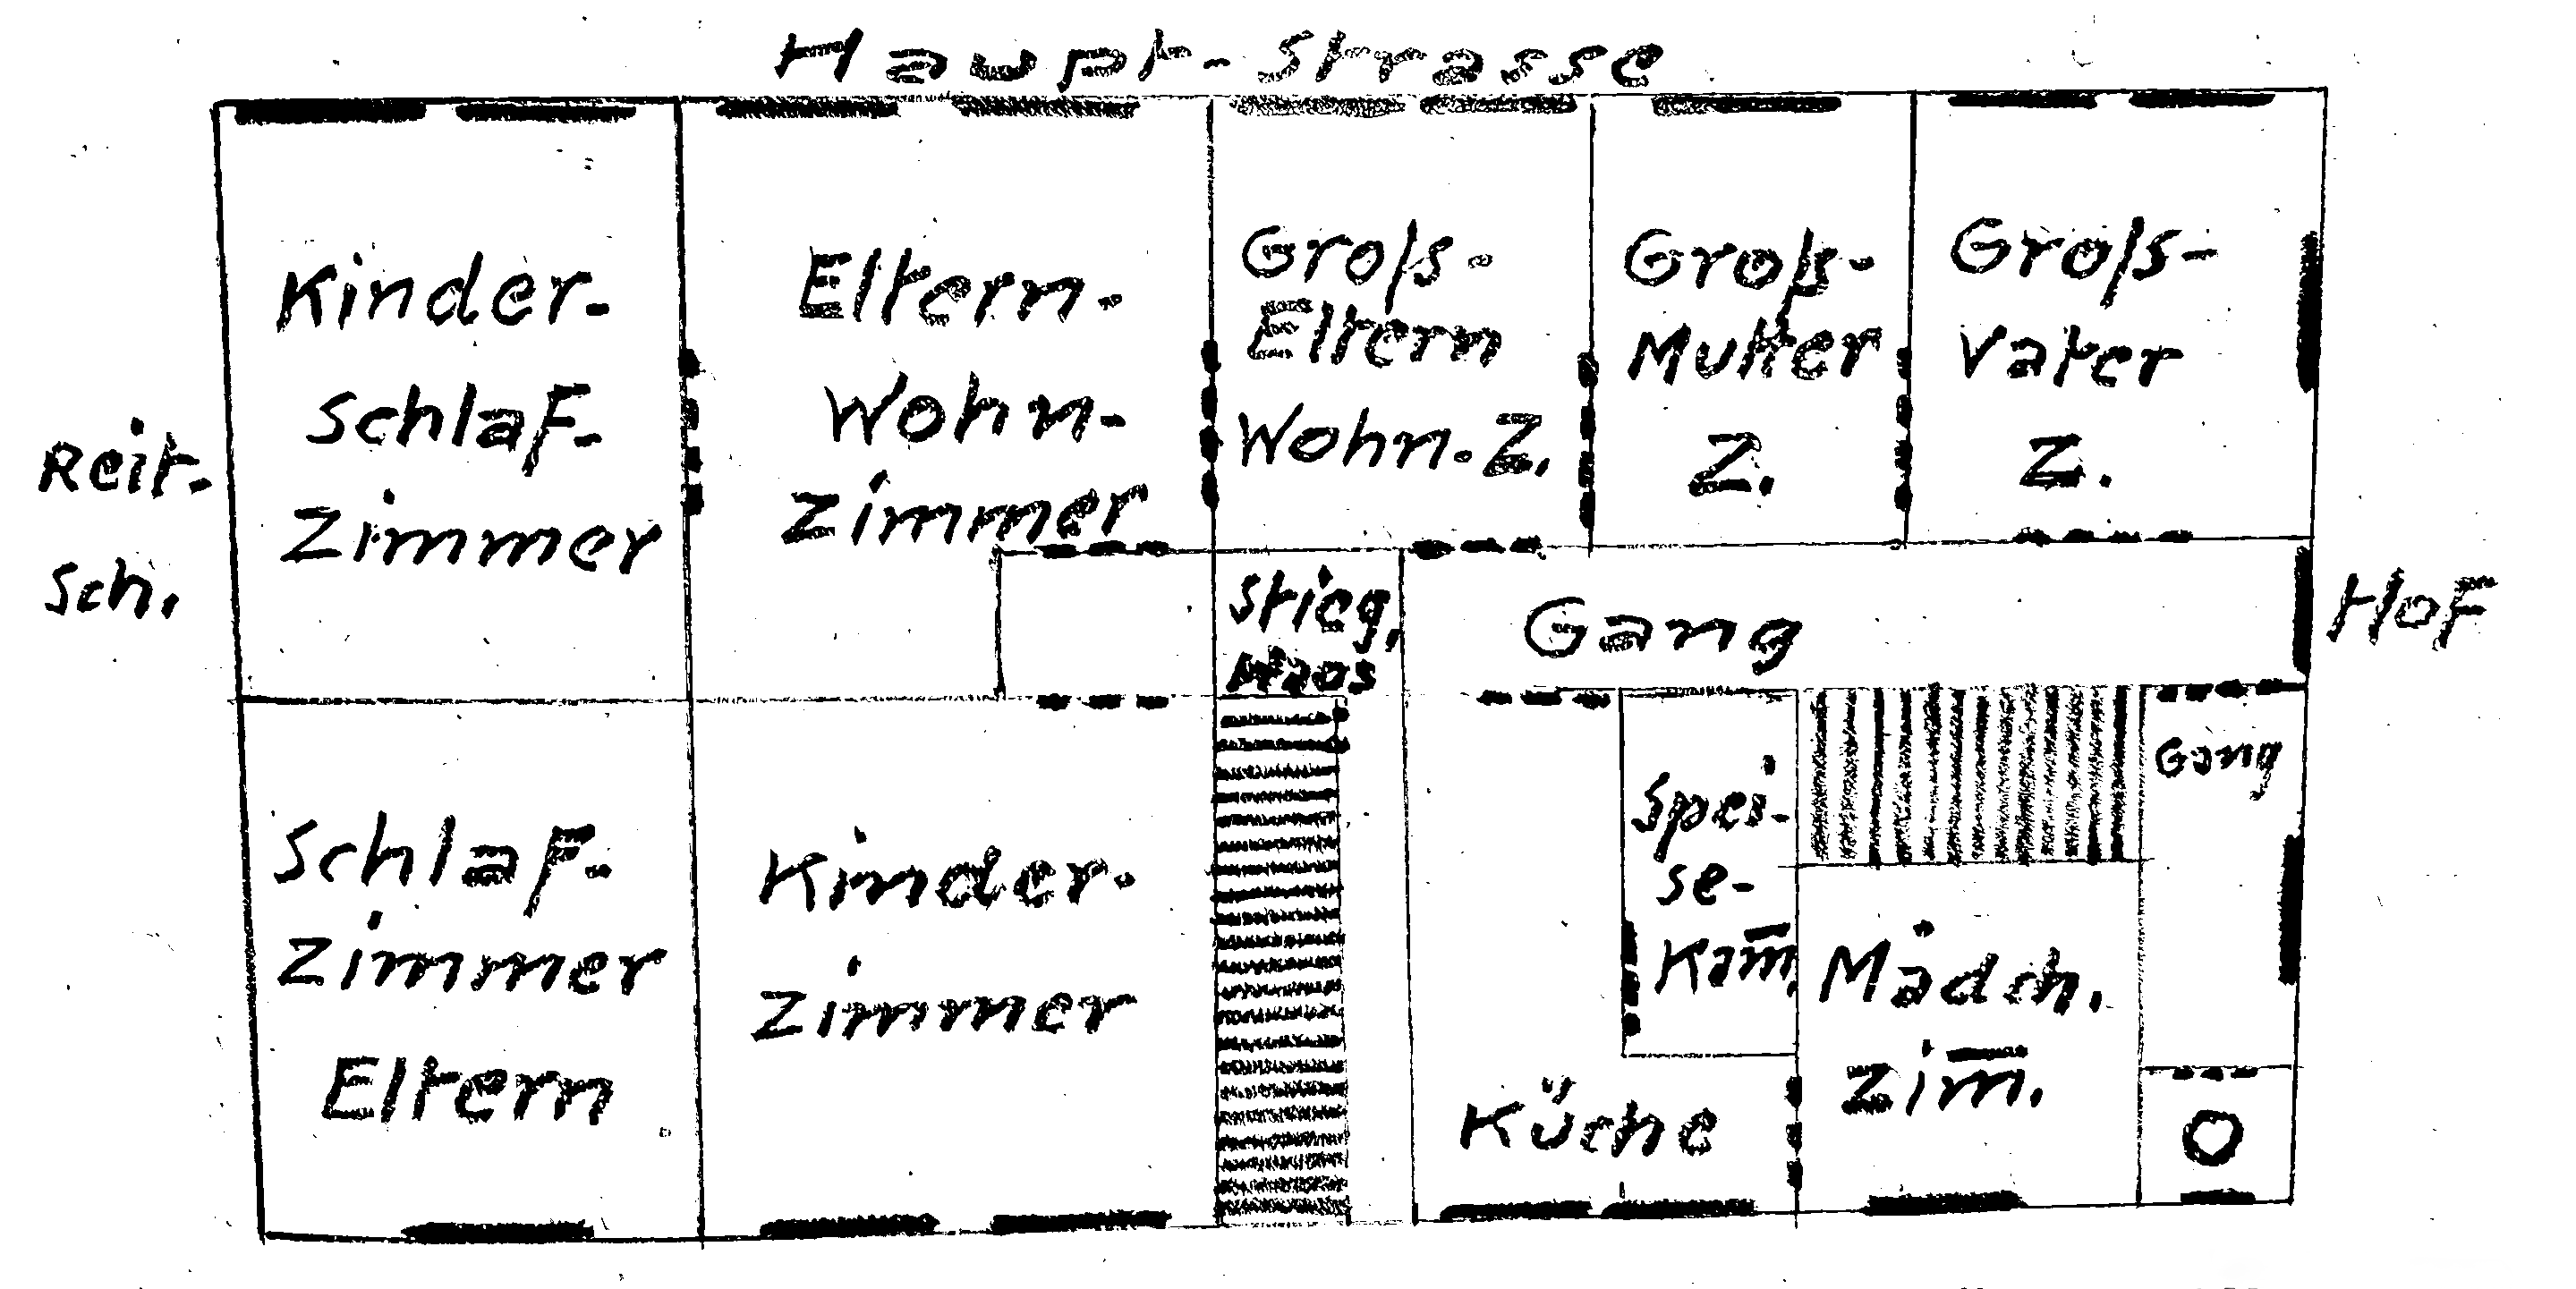
\includegraphics[width=1\linewidth]{Grundriss Wohnung Kleinheubach.png}
    \caption{Unsere Wohnung mit den Großeltern zusammen bis 1901. Nach dem Tode der Großeltern bewohnten wir nur noch deren Wohnung allein bis zum Jahre 1907.}
    \label{fig:Grundriss Wohnung Kleinheubach}
\end{figure}

Im Jahre 1892 wurde uns ein drittes Schwesterchen geboren, unser Karolinchen, ein gesundes, munteres Kind. Doch durfte es nicht lange unter uns weilen. Nach mehreren Monaten entwickelte sich durch Erkältung eine starke Schleimbildung, die einen baldigen Tod verursachte. Der Schmerz der Eltern war groß. Er wurde überwunden in den Tröstungen unserer hl. Religion. Die Mutter sagte zu uns: Jetzt ist es in die Schar der Engel aufgenommen. Auf einem Grabsteinchen ließen die Eltern die Inschrift anbringen: \textit{Leb wohl, du liebes, gutes Kind, bis wir einst wieder bei dir sind}.
Von dieser Zeit an war lange unser häufiger Gang zum Friedhof mit der Mutter, der Vater war meist dienstlich verhindert. Dort in der Nähe war ein größerer Wasserdümpel. Wir holten hier das Gießwasser für das Grab. Da gab es Unterhaltung für uns. Die lustigen Fröschlein streckten ihre Köpfchen hoch und ließen ergötzende Laute von sich hören. Immer wollten wir welche fangen, doch gelang es uns nicht. Die Mutter hatte Mühe, uns vom Wasser wegzubringen. Rasch verging da die Zeit, wir mussten nach Hause.

Gerne hörten wir auch stets den Erzählungen der Mutter und Großmutter zu aus ihrer Jugendzeit. Besonders denke ich daran, da ich, wie später noch folgt, mehrere Jahre in Wörth a. Main zubrachte und viel die Grabstätte eines Pfarrers \textit{Anton Saalig} besuchte, der Onkel der Großmutter, wie letztere sprach.

Als wir in Baumanns Haus wohnten und ich noch jung war, lag meine Mutter immer zu Bett (sie war gichtleidend). Sie hatte ein kleines Hündchen und wenn dasselbe lebhaft wurde und anschlug, war etwas Besonderes. Da läutete die Großmutter und als eines ins Zimmer trat, sagte sie: Schau einmal zum Fenster hinaus, es wird der Wörther Onkel kommen und richtig, der Onkel fuhr bereits mit seinem Gespann über das Brückchen (am Dorfeingang).*-Welch schöne Stunden mögen sie dann gemeinsam verlebt haben.-Am 1.Mai, 1893 wurde ich in die Volksschule aufgenommen mit,,Fritz Abb,Bertha Schell und Marie Rebel.Als Lehrerin hatten wir die ehrwürdige Frau M.Jgnatia Raßhofer,die in Anbetracht der wenigen Kinder,36 zusammen,alle Klassen in einem Raum leitete .Unser Religionslehrer war der damalige Schloßkuratus H.H.Pater Kajetan Kiefl vom Franzis-ianerklpster auf dem Fngelberg.Er war für uns ein gefürchteter Mann, alle in schon durch seine große Erscheinung.Mehr zur Strenge neigend,trat immer wieder das sogenannte,,Spanische Rohr'‘in Anwendung, umsomehr, als er auch teilweise die,von der Lehrerin übergebenen Bestrafungen übernahm.Geschadet haben diese Züchtigungen jedenfalls nicht. Manchmal mußten wir auch ein selbstgeschriebenes Schuldbekenntnis den Eltern zur Unterschrift vorlegen, dann bekamen wir meistens nochmals eine Lektion als Denkzettel .Die Schulteit hatte ja auch viel Schönes.Große Freuden wurden uns bereitet durch das fürstliche Haus »besonders durch die Geschenke am Weihnachtsfeste ,welche im Schulhause mit einer Feier verbunden,zur Verteilung kamen. Am Fronleichnamsfeste mußten wir mit Flasche versehen zum Schloß kommen,um dort dieselbe mit Wein gefüllt zu erhalten,auch wurde uns eine ausgiebige Portion Kuchen verabreicht.Jmmer gab es einen Anlaß zur Freude.Am 8.Nov.l893 war die Vermählung von Prinzessin Maria Theresia mit Don Miquel von Braganza,ein großer Festtag.Der Vater hatte bereits mehrere Wochen vorher alle möglichen Vorbereitungen in der Küche zu treffen,da viele Herrschaften, hauptsächlich von Bayern und Oesterreich erwartet wurden.Fr war wenig zu Hause .Am Hochzeitstag selbst machten wir uns,Maria und ich wohl in der Nähe der Schloßküche zu schaffen.Fs fügte sich,daß uns die Diener in den Marmorsaal brachten und uns ein Platz chen als Zaungäste anwießen an den Serviertischchen, die zwischen den Fenstern angebracht waren. Erstaunt schauten wir all‘diese Pracht,die heri>-liehen Kleider und die feinen Uniformen.Als dann in einer Fcke des Saales die Militärkapelle einsetzte »wurde es uns bald unheimlich.Jedenfalls schlichen wir uns zeitig wieder fort,wohl fühlend, daß wir in solcher Umgebung nichts zu schaffen hatten.Häufig brachte uns der Vater etwas aus der

  Schloßküche mit nachhause oder schickte ein Küche nmädchen. Oft kamen wir auch selbst hin und erhielten,wenn der Vater guter Dinge war,manche Süßigkeiten. Auch dem Großvater durften wir manchmal das Frühstück bringe n;er hatte dortselbst sein Arbeitszimmer.Einträgliche Besuche waren für uns auch bei der Beschließerin und in der Kaffeeküche. Bei den Männern hatten wir da wenig Erfolg,es kam nur zum Scherzen und Lachen.-Zu Hause weilten wir gerne bei den Großeltern.Sie waren so gut zu uns. Während uns die Großmutter in ihrer mütterlichen Art viel mit praktischen Belehrungen bereicherte , wußte uns der Großvater mit Erzählungen aus der Biblischen Geschichte zu fesseln.Mit Vorliebe hörten wir seine Heise-Erlebnisse mit dem Fürst,Baron Korff etc. in Jtalien und Palaestina.Ab und zu wurden wir auch angehalten,den Rosenkranz mit ihnen zu beten.Wir suchten sie aber auch auf,wenn wir etwas angestellt hatten,um Schutz vor Strafe bei ihnen zu finden.Der Vater wurde dann von der Großmutter beschwichtigend beeinflußt .Manchmal sagte er aber auch:Ja,Schwiegermutter,das geht nicht—wenn sie nicht brav waren,müssen sie gestraft werden.Er war da rechtschaffen aber auch sehr gut. War die Zeit zum Pilze und Schwämme suchen,durften wir mit in den Wald.Schöne Exemplare brachte er gerne den Herrschaften,die sie mit Vorliebe aßen. Zur Mutter fühlten wir uns ja mehr hinge zogen, sie hatte ein ruhiges und liebevolles »Vesen.Saß sie ab und zu am Klavier »lauschten wir gerne und konnten nicht genug bekommen.Bald sagte das Eine:Mutter spiel noch einmal-Der Vöglein Abendlied Mutter,-Das Lied einer Jungfrau oder den Mazurka.Diese Stücke hörten wir am liebsten.-Einmal kam der Vater __ nachhause und sagtes »Dieser Tage muß ich nach Bron— bach und Geschirr dort zusammensuchen für Schloß Fischhorn,bezw.Haid.&s bestand noch keine Bahnverbindung nach Wertheim und so veranlaßte er den Heubacher Lohnkutscher, den:Amends Schorschle * ihn dahin zu bringen.Die Mutter überlegte,-dann sagte sie zum Vater:Du könntest eigentlich die Buben mitnehmen. Da war es aus mit uns »Unsere Freude war unbegrenzt. Wir konnten bald den Morgen nicht erwarten,stand uns doch,da wir außer den Nachbarorten noch nichts gesehen,eine große Reise bevor.Schon in früher Morgenstunde kam der Wagen angefahren.Der Schor-schle richtete den Sitz zurecht und der Vater nahm Platz.Jakob durfte zu Vaters Rechten sitzen, ich wurde links platziert.Die gute Mutter hüllte uns noch fest in Decken ein,es war ziemlich frisch. Die Lederscheibe wurde eingehängt und die Fahrt ging los über Miltenberg-Bürgstadt-preudenberg bis Mondfeld.Da glaubten wir uns schon in einer anderen Welt.Hier wurde das Frühstück eingenommen im Gasthof,Zur Kanne’Der Vater ließ sich Bier vorsetzen und wir bekamen Milch mit Brot.Doch schon konnten das Weiterfahren nicht erwarten und waren wieder ₐuf der Straße.Nₐ<»h. einigem Aufenthalt gings über Wertheim nach Schloß Bronnbach.Aufs Freundlichste wurden wir von dem Verwalter begrüßt.Der Vater erledigte bald darauf seine Angelegenheit und überließ uns der Obhut von Frau Böttigheimer,der Frau des Verwalters,die uns durch gute Bewirtung und Unterhaltung zu fesseln wußte .Wir durften das Schloß besichtigen und so eilten die Stunden rasch dahin.Gegen Abend fuhren wir wieder heim.—Ks kam die Zeit,wo ich zum Ministrantendienst zugelassen wurde .Das Spielen in freien Stunden wurde mehr eingeschränkt, dafür mußte das Lernen der Meßgebete etc.eingeschaltet werden.Mühe war schon damit verbunden, bis das Hersagen der lateinischen Worte funktionierte.Doch hatte ich Freude daran.Die reiche

Ablenkung im Kirchenjahr brachte viel JnterresSantes für die Ministranten »besonders in der Oster-zeit hatten wir es wichtig.Leider ist mir" ein schönes Buch vom hl• Josef beim Angriff auf Würzburg verbrannt.Als Gedenken schrieb die Großmutter hi— nein:Zur Erinnerung an den 6.Mai, 1894,wo du zum ersten Mal am Altäre den Dienst der Engel versehen hast.Von deinen Großeltern Josef und Anna Rauner. Gerne gingen wir auch mit den Eltern,bezw.mit der Mutter allein auf den Fngelberg. Jhre ,wohl vielen Gebets anliegen hat sie der Gottesmutter dort anvertraut ir Kinder hatten nicht die Ausdauer in der Kirche und drängten nach dem Klosterstübchen, wohin sich die Mutter mit uns ^egab.Der gute Bruder Johannes(ein Münchner)wußte uns stets zu erheitern." ir hörten ihn gerne erzählen.Gut mundete uns das bekannte Klosterbrot mit Butter und Käse. Zum heimgang gerüstet,gings rasch die vielen Treppen hinunter.Die Mutter konnte uns natürlich nicht einholen und wir mußten geduldig warten.Erwähnen möchte ich auch unsere herrlichen V’aldspaziergänge, vor Allem zu den Heunensäulen-und-Steinen,zum Galgen und Strohtempel.Mit Bevorzugung suchten wir Laudenbach auf,dort wohnte eine befreundete Familie unserer Eltern. Sie hatte eine Gastwirtschaft.Wichtig war uns jedoch der Park des Baron von Fe ehe n-bach und wir erhielten stets F'inlaß.Unter einer großen halle waren die Turn-und-Schaukelgeräte der Kinder,da belustigten vir uns gerne .Wir ergingen uns aber auch mit Lust in dem,mit dichten Nadelbäumen angelegten Teil des Parkes,der wie ein «Irrgarten anmutend,herrlich gepflegt war.-Kam die Beerenzeit, durften wir an schulfreien Tagen zum Pflücken von Heidelbeeren,Himbeeren und Brombeeren mit den Mädchen in den Wald. Je des von uns hatte an einer Leine einen Becher hängen,Marie und Lonchen trugen Körbe ,Firner und Vesperbrot etc.Da wir den ganzen Tag draußen waren,kämeh wir gegen Abend müde he im, doch meist mit vollen Körben und Eimern. Am 20.August,1896 wurde unser lieber Fritz geboren. Wohl tags darauf gingen wir in kleinem Zug zur Kirche zur hl. Taufe-wir Kinder voraus,der Vater mit der Amme und dem Kind hinterher .Ca. ein Jahr später brachte mich der Vater in die Real-und-Handelschule nach Miltenberg.Die schöne Kinderzeit daheim hatte ihren Abschluß gefunden.Der Weg zur Schule dauerte über eine Stunde .Schulstunden waren es mehr wie bisher,auch die Hausaufgaben nahmen längere Zeit in Anspruch.Zum Spielen blieb nicht mehr viel Zeit. Morgends,ca.6.45 sammelten wir uns(die Schüler.welche das Gymnasium und die Realschule besuchten)am Parke ingang .F in passender Zug ging nicht und wir mußten den Weg zu Fuß zurücklegen.An Regentagen oder bei Winterkälte war derselbe nicht gerade schön.Ab und zu waren wir auf dem Heimweg vom Glück begünstigt »wenn uns ein Fuhrwerksbesitzer auf seinem Wagen mitnahm.War die Witterung zu ungünstig im Winter,durfte ich bei einer bekannten Familie in Miltenberg bleiben und kam dann erst am Wochenende nach Hause.Diese Unterkunft sagte mir nie zu,

 alles war primitiver wie daheim,der liebevolle Umgang fehlte-ich sehnte mich stets nach dem Elternhause .Einmal sollten wir bei hohem Schnee den Weg zurücklegen,da fügte es sich,daß ein Kutscher mit seinem Schnee schlitten den Weg durch den Park bahnte und uns erlaubte , mit zufahren.Ein großes Brett wurde darauf gelegt,wir hatten alle Platz und waren guter Dinge.Die vor gespannten, Braunen’hatten einen guten Trab und es ging lustig durch den Schnee. Bald hatten wir den Aus gang des Parkes erreicht, ereilte uns das Ungeahnte.Durch den hohen Schnee nicht sichtbar,flog der Schlitten gegen einen Randstein und wir saßen plötzlich im Schnee .Nur dem Kutscher dürfte das Lachen geblieben sein,als wir,unsere Bücher zusammensuchend,aus dem Schnee uns erhebend, die Plätze wieder einnahmen.Eg war keinem von uns etwas dabei passiert.-Nur drei Jahre besuchte ich die Handel schule .Während dieser Zeit entschloß sich auch Maria im Kloster St.Maria Stern in Augsburg als Schülerin einzutreten.Am 17.Juli,1899 starb mein guter Großvater.Es war ein recht schmerzlicher Verlust,wir hatten ihn sehr gerne.-Jm Frühjahr,19ol fuhr die liebe Mutter mit mir nach Würzburg,wo ich eine Lehrstelle im graphischen Gewerbe erhalten sollte und großes Jnterresse dafür zeigte.Von Vaters Vorhaben,seinen Beruf zu ergreifen,wurde abgesehen. Der erste Gang der Mutter war in die Bibraanstalt, um ehrw.Frau Neomisia,die ihre Kandidatur zeit in Kleinheubach verbrachte , zu begrüßen .Darauf wurde ich im Lehrlingsheim bei der Augustinerkirche eingeführt.Nachdem die Mutter ihre Mission erfüllt hatte,fuhr sie wieder he im.Der Vorsteher und Präses des Heims war Herr Domvikar Meckel .Er bemühte sich,in der lithographischen Anstalt der Univer-sitäts drucke re i von H.Stürtz um Aufnahme für mich. Doch waren schon genügend Schüler vorgemerkt und ich mußte noch gegen zwei Jahre warten.Während dieser Zeit besuchte ich die höhere Zeichen-und Mo de lier schule .Mit Professor Gaab und Bildhauer Los ter waren mir tüchtige Lehrer gegeben. Jm Lehrlingsheim war ich gut auf gehoben.Es wurde von Klosterfrauen aus dem Kloster St .Maria Stern geleitet. Auch Schüler des Gymnasiums und der Maschinenbauschule waren dort auf genommen. Wir hatten einen Präfekt,der für Aufsicht und Ordnung zu sorgen hatte .Ein gemeinsamer Speisesaal war zugleich auch unser Aufenthalts raum in freien Stunden.Zum Schlafen waren wir in zwei Räumen eingeteilt,die durch das Präfekt zimmer getrennt waren. Je der Schüler und Lehrling bekam einen Schrank zugewiesen, in welchem neben den Kleidern auch die sonstigen Habseligkeiten untergebracht waren und im langen Gang seinen Platz hatte .Für die Schuhe gab es einen gemeinsamen Schrank,in welchem jeder sein Fach hatte »Dort wurden auch die Schuhe gereinigt. Morgens 5.^0 war erstes Glockenzeichen zum Aufstehen, um 5 »4-5 gemeinsames Morgengebet .Um 6 Uhr gingen wir mit dem Präfekt zum Anhören der heil. Messe auf die Empore der Augustinerkirche.Nach Gottesdienst war Frühstück .Wer sich eine kleine

  Verfehlung zu schulden kommen ließ,erhielt statt 2 Semmel ein Schwarzbrot .Dann ging Alles zum Beruf ,bezw.die Schüler zur Schule.Der Mittagstisch war um 12.15.Nach dem Abendessen um 7 Uhr konnten die Lehrlinge zum Spiel zusammen sein,ebenso die Schüler, sobald ihre Lernzeit vorüber war .Um 8.45 war gemeinsames Abendgebet,um 9 Uhr mußten wir zu Bett .Sonntags gingen wir wieder zusammen zum Gottesdienst und zur Nachmittags andacht, im Übrigen hatten wir frei.Am 9.August,1901 starb unsere lb.Großmutter.Bald darauf mußten die Litern eine Wohnung auf geben und be hielten die Wohnräume der Großeltern bei,da wir uns auch hauptsächlich darin aufhielten.Daheim wurde es einsamer, wir hatten nur noch unsere Maria Moor als Hilfe.Am 29*März,19O5 konnte ich endlich meine Lehrzeit in der Universitätsdruckerei von H.Stürtz beginnen. Die selbe wurde nur auf drei Jahre fest-gesetzt,während im Allgemeinen 4 Jahre vorgeschrieben waren.Jetzt hatte ich Gelegenheit in allen Zweigen der Lithographie ausgebildet zu werden. Jm ersten Lehrjahre mußten wir noch an einigen Tagen der Woche vormittags die Zeichenschule besuchen.Die lithographische Abteilung war damals mit ca.55 Zeichner und Zeichnerinnen besetzt,die in zwei langen Reihen mit ihren Arbeitspulten den Saal füllten.Am Anfang des Raumes hatte der Obe rlithograph( abge te ilt) se in Arbe itsbe re ich, am Ende der Faktor.Die Lithographie machte einen vornehmen Eindruck auf mich.Dem ersten Zeichner, der stets in schwarzem Frack an seinem Pult,hinter dem Oberlithograph saß,wurde ich zugeteilt.Da konnte ich Vieles sehen und lernen.Abwechslungsreich war ja die Tätigkeit in der ganzen Abteilung. Plakate und Diplome wurden hergestellt»stets Teppich-Zeichnungen,wozu die Original-Teppiche auf großen Gestellen auf gehängt waren, ständig wurden medizinische Zeichnungen angefertigt für die Studienwerke der Universität,daneben Zeichnungen für Buchschmuck,Gravuren in einfacher bis zu feinsten Ausführungen,Zeichnungen für Geschäftskata-loge nach Originalen u.s.w.Lange Zeit nahm der Tauben-und Hühnerkatalog in Anspruch.Fr brachte besondere Ablenkung.Morgens wurden die Tauben-bezw. Hühnerkäfige aufge stellt .Die benötigten Tiere für den Tag wurden eingesetzt und abends wieder in den Hofraum geschafft .Besonders lebhaft wurde es, wenn die Hähne ihr »Kicke ricki * schmetterte n.Der Oberfaktor,ein Hühnerfreund nahm die Fütterung vor.Ab und zu kam der Chef-Geheimrat Stürtz allein oder mit Bekannten und Geschäftsfreunden in den Bet rieb.-Gegen Fnde meiner Lehrjahre zählte ich wohl auch zu den ältesten Jnsaßen im Lehrlingsheim und erhielt dort ein ^inze 1 zimmer ehe n, auf welches ich nicht wenig stolz war,da nur der Präfekt ein solches hatte, allerdings größer und gut eingerichtet.Bald darauf lernte ich einen jungen Mann kennen,dessen Vater bei der Polizei Anstellung hatte.Diese Familie wollte mich in ihre Behausung aufnehmen und so schied ich, 19 jährig,

  vom Lehrlingsheim.-Jnzwiseben verließen die Fltern ihre Dienstwohnung und bezogen ihr neues Anwesen in der Friedenstraße,am 17.Juni, 1905.Am 29.März, 1906 war meine Lehrzeit beendet.Der Vater wollte mir eine weitere Ausbildung zuteil werden lassen und so durfte ich anschliesend nach München.Zwei meiner Rollegen(Gerhard und Knittel)kamen kurz vorher dorthin zu technischer Vervollständigung.An diese dachte ich und stellte in Frage,ob ich ihnen in dieser Großstadt begegnen würde.Durch den Bruder einer dort ansäßigen Verwandten von Mutters Seite (Anna Steiner)erhielt ich ein möbliertes Zimmer in der Regerstraße (Außenbezirk) im 5.oder 4.St. Vom Fenster aus konnte ich die Gebirgskette bei klarem Wetter sehen.Nun gings daran,einen geeigneten Schulbetrieb zu suchen.An einer Mal-und Zei-chenschule in der Herrnstrasse konnte ich Aufnahme finden bei Professor Dietl.Dort bestand meine Arbeit in Zeichnen nach der Natur.Daneben besuchte ich Akt-und PorträtZeichenkurse »ebenso Perspektive-und Anatomiekurs(f.plastische Anatomie).Unser Ziel ‘heim Landschaftszeichnen bildete die Au.Dort konnte ich feststellen,daß meine erste Arbeit ein Bild darstellte ,welches ich von entgegengesetzter Seite bereits einmal nach Vorlage in Würzburg gezeichnet hatte.Die Vorlage war von Kunstmaler Bernhard Wenig,der mir in späteren Jahren befreundet wurde.Meine Verköstigung mußte im Gasthaus sein, da meine Hausleute sich nicht damit befaßten.Am Jsartorplatz wählte ich mir eine Gaststätte .Kurze

- Zeit nach Bezug meines Zimmers hörte ich im Vorplatz den Namen meines Kollegen Gerhard und richtig fanden wir uns zusammen,als er mit dem,neben mir wohnenden Schneider eine Unterredung hatte. Ueberraschung und Freude überkam uns beide .Nach seiner Wohnung fragend,sagte er mir:«Ich wohne gerade gegenüber'Wo steckt denn der Knittel,sagte ich.Der wohnt ein Stück weiter oben,kam es zurück und ich konnte von meinem Fenster beide Häuser sehen-»Sonderbares Zusammentreffen'Während meines Schulbesuches in der Herrnstrasse wurde eine Sonderfahrt-Münchner Kunstschüler-zur,Gewerbe-Aus Stellung in Nürnberg,durchgeführt,an welcher ich mich beteiligte.Dortselbst erwartete mich mein 1b. Vater, der auf seiner Dienstreise nach Fischhorn einen Tag in Nürnberg verweilte .Die vielfachen Ausstellungsgegenstände auf dem grossangelegten Platz ermüdeten sehr bei ihrer Besichtigung. Vater und ich trennten sich von meinen Lehrern und Kollegen und gingen zu dem Gasthof,in welchem wir auch Nachtquartier bezogen.Am kommenden Tag setzte der Vater seine Heise fort.Mit den Kollegen besichtigte ich noch die Sehenswürdigkeiten der Stadt »besonders das,Germanische Muse um .Wir fuhren gegen Abend wieder nach München zurück .Später wechselte ich meine Wohnung und zog in die Frauenstrasse »nicht weit von der Schule entfernt und wohnte bei einem Poliaei-Wachtmeister.Dort wurde ich häufiger von Bekannten besucht.

-Wenn ich mich auch nicht viel an den Bierabenden

 beteiligte,soll doch ein lustiger Aufmarsch erwähnt sein .Fines Tages kam ein Kollege zu mir mit einem Karton zum Sammeln.^s sollten Lebensmittel zusammengebracht werden für ein Abendessen im oberen Saal des Hofbräuhauses.Jch beteiligte mich mit ein Paar Würstchen,da ich erst eine Sendung von zuhause erhielt.An dem bewußten Abend war gemeinsames Antreten.Unser Führer ging mit seiner Kiste,die alle möglichen Speisen und Raritäten enthielt voraus und wir mußten im Gänsemarsch folgen, wo hin er uns leitete.So war er im Saal angelangt.Natürlich gut besetzt’.Bs genierte ihn nicht .Zwischen den Tischreihen war nicht gut durchzukommen,so gings über Stühle und Tische,wenn auch Maßkrüge und Teller bedenklich wackelten zum allgemeinen Gaudium,bis wir uns irgendwo niederlassen konnten.Dort wurde die Kiste auf den Tisch gesetzt und es ging an's Verteilen. Jm Hofbräuhaus konnte man das ja alles machen.Für mich waren das ungewohnte Mannöver,aber man tat mit. Auch von meinem Hausherrn,dem Herrn V/achtmeister ein heiteres Erleben.Fr ging,wie so oft,in feiner Uniform und mit Helm zum Dienst.Kaum die Wohnung verlassen, gab es großen Radau im Stiegenhaus .Wir hatten eine Rundtreppe und der strenge Herr rutschte von Tritt zu Tritt die Stiege hinunter,der Helm voraus .Es war wohl Alles auf den Beinen, der Herr Wachtmeister kam aber ohne Verletzung durch.Vielleicht hatte erte seiner vollen, gut genährten Entscheinung zu danken.Bier hat er stets gern getrunken,doch konnte man keine Schlüsse ziehen.Während

“ich dort wohnte,kam ein Landsmann von mir nach Mün-chen,um sein medizinisches Studium zu vollenden. (Fritz Meyer), Jetziger Arzt von Amorbach.Von dieser Zeit an war ich viele freie Stunden mit ihm beisammen.Wir machten Ausflüge in's Jsartal,zum Starnberger See »besichtigten eingehend die Münchner Sehenswürdigkeiten und besuchten öfter die Theater. Sonntags gingen wir zusammen zum Gottesdienst, hauptsächlich in die Michaels-Hofkirche,wo Sänger und Sänge rinnen, wie auch das Orchester des Hoftheaters zur Verherrlichung beitrugen.inzwischen verließ ich die Schule an der Hermstrasse und verlegte mich besonders auf Akt-und Porträtzeichnen. Mein Arbeitsbereich war Jetzt im Weinhold-Schildknecht-Atelier in der The re s ie ns t rasse .Mein Landsmann Meyer hatte inzwischen seine Semester vollendet und verließ München.Doch stellte sich bald Fr-satz ein.Von Kleinheubach erfuhr ich,daß der Sekretär des Fürsten Löwenstein für einige Zeit nach München kommen werde betr.Uebe rtragung der Anti-Duell-Liga, was Baron von Kramer-Klett übernehmen wollte .Wir traten auch bald in ein freundschaftliches Verhältnis.Philipp Schach hatte Verwandte in der Regerstrasse (mein erstes Zuf luchts vie rte 1) die ihm ein Zimmer in der Nähe besorgten.Kaum glaublich,als ich ihn besuchte,sah ich,daß er mein erstes Zimmer bewohnte .Wir waren erstaunt, ob solcher Vorkommnisse .Bald kam der Zeitpunkt,zu dem ich München zu verlassen gedachte .Vorher wollte ich mich noch einige Zeit praktisch betätigen,was ich

  in der Kunstanstalt von Hubert Köhler erreichte.¹ Da der Portier des Barons v.Kramer-Klett,den Philipp inzwischen kennen lernte,in der Nähe meines Tätigkeitsbereiches wohnte,erhielt ich bei ihm ein Zimmer in der Zieblandstrasse.Mit Philipp trat ich bald in ein intimeres Verhältnis .Wir wohnten zwar entgegengesetzt,doch hatten wir stete Verbin-dung,trotz der ^ald einstündigen Entfernung.!¹ ines Abends besuchte ich ihn in der Regerstrasse .Beim Abschiednehmen wollte er mich kurz begleiten,um sich noch ein Bier heimzuholen.Es war ein warmer Herbstabend .So nahm er seinen Krug und ging, wie er war,ohne Kragen,ohne Kopfbedeckung,in Hauspantoffeln mit,war ja der Bierschalter ganz nahe.Die Abendluft sagte ihm zu und er ging weiter mit.Wir kamen schließlich zum Gärtnerplatztheater.Jedenfalls hatten wir uns viel zu erzählen und setzten uns dort einige Zeit auf eine Bank.Nicht genug, ging seine Begleitung weiter und wir kamen schließlich bei meiner Wohnung an.Fr ließ sich überreden und wir tranken statt Bier einen Tee auf meinem Zimmer.Zur nächsten Strassenbahnhaltestelle begleitet,fuhr er wieder heim.Jm Frühjahr, 19o8 verließ ich München,um zunächst kurze Zeit bei den 1b.Eltern zu verweilen.Ein Verwandter der Mutter,Anton Steiner,bei der Polizeibehörde in Trier tätig,gab mir Veranlassung,dorthin zu kommen.Meine Schwester Jose fine weilte zu Besuch bei ihm, sodaß mein Beschluß beschleunigt wurde,auch zog mich die Stadt mit ihren historischen Sehenswürdigkeiten an.Bald verließ ich wieder die Eltern.Jn Trier angekommen, fand ich gleich Beschäftigung in der graphischen Anstalt von Schaar und Dathe.Die Abteilung wurde getrennt geführt.Es arbeiteten nur drei Herrn und ein Fräulein.Ein Jahr teilte ich mit ihnen die anfallenden Arbeiten,die in der Herstellung von bunten Ansichten aus England etc.bestanden.Jn der Freizeit sorgten schöne Spaziergänge in's Moseltal und in die Eifel für reiche Ablenkung,die ich ja auch bei Anfertigung einer Adresse zur Silberhochzeit unserer guten Eltern fand.Diese Arbeit konnte ich durch Entgegenkommen meiner Hauswirtin »Frau Jungblut'die mir ein grösseres Zimmer,neben dem meinen zur Verfügung stellte,gut zu Ende führen.Diese Jubiläumsadresse war mir vor dem Heimgänge der guten Eltern übergeben worden und wurde ,wie so vieles Andere beim Luftangriff auf Würzburg,am 16.3.45 ein Raub der Flammen. Al Imäh— lig wurde das Verlangen in mir wach, wie der zur Firma Stürtz zurückzukehren und ich früg an,ob ich mit einer Aufnahme dort rechnen darf .Nachdem die Mitteilung eintraf,daß ich jederzeit wieder eintreten könne »meldete ich mich für den Monat Mai an.Bei meinem Abschied von Trier,ließ es sich Frau Jungblut nicht nehmen,trotz der frühen Morgenstunde ,mir noch ein fürstliches Frühstück zu richten.Es herrschte noch Dunkelheit,als ich das Haus verließ.Vor meiner Heimfahrt besuchte ich noch die alte Stadt Luxemburg.Die Eltern freuten sich,wie stets auf ein Wiedersehn,so blieb ich

.bis Mitte Mai bei ihnen.Folgend wandte ich mich an die Firma H.Stürtz in Würzburg und fand freundliche Aufnahme .Ein gewohntes Geschäft ging voraus, das Zimmersuchen,was damals mit keinen Schwierigkeiten verbunden war,aber ungünstig ausfallen konn te »wenn man nicht in die rechte Familie geriet.Jn der äuseren Huttenstrasse habe ich günstige Wohnung gefunden bei einer Musikdirektorswitwe Wilhelm,die durch ihr äußeres Auftreten so recht defe verstorb.Fhe gatten in seiner Possition vertreten konnte.Jch hatte volle Verpflegung bei ihr,auch wußte sie sich gut zu unterhalten.-Jn unserer Lithographie war ich gleich wieder zu Hause,die Arbeiten waren mir aus früheren Jahren nicht neu. Jn meiner Freizeit suchte ich meinen Bekannten, Josef Hers am auf,bei dessen Fite rn ich erstmals wohnte und hatte durch ihn reiche Ablenkung.Als Musikfreund stellte er ein Sängerquartett zusammen, dessen Mitglieder mir liebgewordene Bekannte wurden.Vor Allen trat ich mit Glasermeister Georg Spengler und dessen Bruder Karl in ein freundschaftliches Verhältnis.Spengler war wohl 10 Jahre älter als ich,doch hat mir sein,etwas väterliches Auftreten mir gegenüber gut gefallen.Die Familie hatte gut christliche Einstellung und manchmal war er mir ein guter Schutzgeist in den Gefahren des Lebe ns. Als meine Hauswirtin eines Tages verreiste und mir ihre erwachsene Tochter,die eigens von Ostdeutschland nach Hause kam,allein in der Wohnung für den Haushalt überließ,war es mein Freund Spengler,der mich,die Gefahren erkennend,

__ davon abhielt,zu Hause zu bleiben.Meine Freizeit verbrachte ich dann hauptsächlich bei ihm bis Frau Wilhelm wieder nach Hause kam.Aus früheren Unterhaltungen durfte man entnehmen,daß sie mich gerne in deren Verwandtschaft gesehen hätte.Doch war es besser so.Die Tochter reiste alsbald wieder ab.Jn dieser Wohnung besuchte mich auch einmal meine Schwester Josef ine, ebenso Philipp Sch. der sich mit ihr zu vermählen gedachte .Am 7.Mai, 1910 war ihre Hochzeit in Kleinheubach.Von diesem Zeitpunkt an besuchte ich sie häufig in der neuen Behausung in Kreuzwertheim.Jmmer freute ich mich auf die Radfahrt am Samstag Nachmittag.Bs gefiel mir zu gut dort.Das Haus,(vorher von einem Prinz bewohnt)war von einem Garten eingeschlossen.Vom Wohnzimmer aus führte eine Freitreppe in den Blumen garten, auf der anderen Seite war der Gemüsegarten.Jn Ersterem saßen wir oft bis spät in die Nacht in dem schönen Gartenhäuschen bei Lampionbeleuchtung;früh erwachte ich bei schönstem Vogelkonzert .-Meine Wohnung in der Huttenstrasse mußte ich bald aufgeben,da die Frau zu ihren Verwandten nach Nürnberg verzog.Jn der Sophienstrasse mietete ich ein Zimmer bei einer Frau Gmelch.Die Frau lebte von dem Erlöß ihrer Mieteinnahmen,das Wohnen dort war weniger günstig. Mein Bruder Jakob,zu dieser Zeit bei dem 11.Feld-Artillerie-Regiment eingerückt »machte sich das Zimmer häufig zu Nutzen,indem er gerne dort sein Mittagschläfchen hielt.Ls kam auch vor,daß er

  über die Zeit schlief und einmal bis zu meinem Heimkomme» vom Geschäft »och da war .Fs blieb ihm licht mehr viel Zeit bis zum Eintreffen in. der Käse ne und er wollte mir wohl Manches »och mitteile ».Wir machte» u»s rasch auf und liefe» de» Weg bis zum Torposten,den wir gerade erreichten, als das letzte Signal zu hören war.Ab und zu besuchte ich ihn in der Kaserne .Meine Zeit war meist beschränkt und so konnte ich, falls Appel Iw ar, das Ende desselben nicht abwarten.Da standen sie in Heih und Glied,davor der gestrenge Herr Feldwebel. Jch schrieb einen Zettel zur Verständigung,hielt inn hoch,daß Jakob denselben sehen konnte und steckte ihn hinter eine auf gehängte Schießscheibe, wo er später abgeholt wurde .Jakob war meist müde,wenn er zu mir kam oder wenn wir zusammen Besuch machten bei den Verwandten,Generalarzt Ehehalt.Dort schlief er einmal während des Essens ein zum allgemeinen Gelächter.Er selbst war ja auch lustig veranlagt und konnte sich recht mit freuen.-Durch meinen Freund Spengler kam ich häufig in die Frankenweinstube St. Kilian.Br hatte aus Geschäftsinteresse manche Gaststätte zu besuchen,dort aber war sein Lieblingsaufenthalt.Zwischen der Schwester des Besitzers und ihm kam ein Verhältnis zustande,das zu einer glücklichen Ehe führte .Es war die erste Hochzeit in Würzburg, an der ich mich beteiligte.Jm Norbertusheim in Zell wurde dieselbe gefeiert .Wir fuhren mit Pferdegespann dahin,doch dauerte es gute Zeit bis die Wagen eintrafen,da ein grosser Kreis von Verwandten

- ymd Bekannten sich einfand.Die Schwestern he sorgten die Küche und die Bewirtung .Fs war ein schöner Tag.Abends fuhren wir zusammen nach St.Kilian und beendeten die Feier.Kurze Zeit darauf war die Vermählung des Bruders Karl Spengler in Schott’s Hotel,an der ich ebenfalls teilnahm.Stets war ich Hausfreund bei diesen Familien geblieben.-Durch Veranlassung eines lieben Bekannten, Nikol aus Sehneider,tätig in der Buchhandlung Bauch verließ ich neuerdings meine Wohnung und bekam ein Zimmer bei dessen Hausleuten,der Familie des Domchordirektors Höller.Wir wohnten dort beisammen in 2 Zimmer bis zu seiner nahen Verheiratung .Fr veranlaßte mich auch dem kaufmänischen Verein Konstantia beizutreten,was noch im Jahre 1912 erfolgte. Hier gab es wieder neue Freunde und Bekannte .Der Vorstand Georg Staab »Prokurist der fränkischen Ge sellschaf tsdruckerei ,mit dem ich in freundschaftliche Beziehungen trat,suchte mich wieder für die Wohnung seiner zukünftigen Schwiegermutter zu gewinnen.Zuvor aber war ich noch einige Zeit mit meinem Freund Luitpold Meyer,als Nachfolger von Nik.Schneider bei Höllers zusammen. Da gab es viel frohe Tage .Die vier Töchter,alle musikalisch,wirkten auch in unserem Verein.8ine davon war die Domorganistin.Fs wäre zu weitgehend, all’die schönen Veranstaltungen Konstantias zu Schilde m, de ren Feste zur Zeit Staabs stadtbekannt waren.Bald war es eine Floßfahrt,bei welcher eine Musikkapelle und ein Faß Bier nicht

   fehlte,dann wieder eine Fahrt mit Luftwagen,Konr zerte und Liederabende mit auswärtigen Kräften u. s.w.Unser Ib.Herr Stadtpfarrer Winterstein fehlte fast bei keiner Kneippe,ebenso sein Kaplan,Herr Josef Ullrich,ein guter Bekannter von mir aus seiner Gymnasialzeit in Miltenberg.Auch unsere Faschingsbälle fanden im Beisein des H.Stadtpfarrers statt.Die Sääle waren musterhaft arrangiert .Die Tänze wurden vorher eingeübt von H.Universitäts— Tanzmeister v.Effner,der dann auch die Tanzleitung übernahm.Nur bekannte ,einwandfreie Damen und Herrn die Damen in Begleitung der Eltern oder Bekannten, wurden zügel assen. Die Damen in feinem Kostüm oder Ballkleid,die Herrn in Frack,Smoking oder Gehrock. Samstags war Kege labend in der Union(Kath. Gesellschaftsbaus, all e Sonntage Zusammenkunft zum gemeinsamen Spaziergang.Es kam zum Umzug zu Familie Storg(Staabs Schwiegermutter)Frl. Lehre rin Storg war bereits verlobt mit Freund Staab .Wieder stand eine Wohnungsveränderung in Sicht .Fs wurde das Echterhaus zu Ende geführt.Die dortigen Geschäfts-Jnhaber,zu denen auch Farn.Storg gehörte ,erhielten eine Wohnung im gleichen Hause.Der mir zugedachte Raum hatte das Maschinenbaus unter sich und so zog ich vor,in eine ruhigere Wohnung zu ziehen. Man hatte auch Einsicht.Jn der Welzstrasse fand ich das Gesuchte .Fs sollte bald wieder anders kommen. Der Mobilmachungstag 1914 rückte näher.Bei dessen Bekanntgabe saß ich gerade mit meinem Freund Meyer in Beer’s Brauerei beim Abendessen.

Zu Hause stand der Rucksack "bereit für unsere Reise nach Jtalien etc.Da wurde nun nichts daraus. Statt dessen fuhr ich nach Hause und von dort mit den "Eltern und Geschwistern gleich wieder nach Wiesen,um unserem 1b.Jakob,der in den nächsten Tagen nach Darmstadt einrücken mußte,das Geleite zur Station Lochborn zu geben.Nach meinen Ferientagen war ich noch einige Zeit in Würzburg.Da der Geschäftsgang aber rapid nachließ »ersuchte der Chef die ledigen Leute,wenn möglich zu ihren Angehörigen zu gehen,da der Aufträge zu wenig.So nahm ich meine Zuflucht wieder zu den Eltern,wissend,dort immer gut auf genommen zu sein.Die Firma zeigte sich ja auch entgegenkommend und schickte allmonatlich einen "Betrag als Entschädigung.Jn "banger Sorge vrurde das Kriegsgeschehen verfolgt.Jako"b mußte bald an die Front und Fritz wurde im Kriegsdienst herangebildet. Jch selbst machte mich ebenfalls mit Einberufung vertraut,doch verstrich noch geraume Zeit bis dahin.Fndlich im Sommer 1915 erhielt ich den Musterungsbefehl .Mit einigen Kleinheubacher Leidtragenden mußte ich mich in Miltenberg,Gasthaus zum-Schönen "Brunnen*einfinden und wurde dem Landsturm zugete ilt .Mitte Oktober gleichen Jahres verließ ich mit zwei Landsleuten Kleinheubach,um "bei dem Bezirkskommando in Aschaffenburg vorstellig zu werden.Dort wurden wir eingeteilt .Als der Zug zusammengestellt war,ging* s mit-Rechts um,vorwärts marsch in Richtung zum Bahnhof .Wohin die Reise ging,wußten wir nicht .Nachmittags kamen wir in Gemünden an.Die Wagen wurden zu längerem Aufenthalt seitlich a^gestellt .Gegen Abend gings weiter in Richtung Schweinfurt,wo wir das Fndziel ahnen konnten. Richtig,bei "Eintritt der Dunkelheit stiegen wir in Bamberg aus und marschierten zur Kaserne in die Pöddeldorfer Strasse .Antreten vor dem Bezirkskoni— mando, ^e rle sen der Namen,Finweisung in die Abteilung war die nächste Folge.Jn unserem Bereich angelangt »stellten wir in dem zugewiesenen Zimmer, wenn man die Räume so nennen soll,unsere Koffer od. Päckchen ab und wurden gleich zum Bad geführt.Nach vollzogener Reinigung erhielten wir ein Abendessen, dann gings auf den Strohsack.Jedenfalls habe ich gut geschlafen.Der kommende Tag begann,wie wohl üblich in der Kaserne mit Kaffee fassen,Darnach erhielten wir Kleider und Schuhe ,Tournister,Gewehr etc.Dann folgte die Zimmer-und Zugeinteilung,darnach waren Unterrichts stunden, denen sich die Hebungen anschlossen.Zuerst in den Zimmern und Gängen der Kaserne,wie überhaupt bei schlechter Witterung.Später wurde der Hof zunutze gemacht .Fs folgten Schießübungen im Wald und Felddienstübungen im Gelände .Während des Marsches wurde stets gesungen,oft Lieder mit geisttödentem Jnhalt.Gottlob war Appetit und Schlaf immer gut,wen mir auch die letzeren Hebungen nicht recht zusagten und ich immer dachte;Vielleicht v erde ich davon noch befreit »bevor wir zur Reserve abt raus portiert werden. Von Zeit zu Zeit war ärztl liehe Untersuchung und nach der Abschlußbesichtigung wurde ich für die Garnison bestimmt,also zum Daheim-bleiben.

Tirotz des Kriegsernstes kam für mich eine ruhige Zeit.Zunächst erhielt ich ’ eisung zur Ausführung von Büroarbeiten .Ein kleines Zimme rohen diente uns (mit mir arbeitete ein Sekretär Kraft von Münnerstadt) als Schlaf-und zugleich Arbeitsraum.3 3 war ein gemütliches Arbeiten.Als man nach einiger Zeit zeichnerische Fähigkeit bei mir vermutete, erhielt ich mit Theatermaler Grahn aus Frankfurt und einem Architekt Süßmeir einschlägige Arbeiten von verschiedenen Seiten.?inige Zeit darnach ■ wurde ich der Schießstube zugeteilt,um die Eintragungen in die Schießbücher zu machen,auch Schießscheiben zum Offizierschießen fertigte ich an und der gl .Eine bleibende Stätte hatte ich auch hier nicht.Man holte mich ins Bezirks—Kommando .Dort wurde mir eine Zeit das Adressenschreiben zugewiesen, dann Telefondienst.Alle möglichen Gespräche wickelten sich da ab,mit militärischen Behörden vor allen Dingen,mit Bekannten und Geschäften. Einmal erlebte ich eine peinliche Situation.Der Adjutand,ein Oberleutnant unterhielt sich oft mit seinem Freund, einem Apotheker. Wie der rief der Apotheker an und ich suchte den Oberleutnant .Mittle r-weile wurde das Gespräch unterbrochen durch ein Dringendes aus Würzburg von Oberstleutnant Werner. Nichtsahnend wollte der Oberleutnant seinen Freund begrüßen,was mit folgenden Worten geschah:»Grüv Gott du altes Sch...Da gäb’s aber ein Donnerwetter beim Oberstleutnant.Natürlich suchte der Oberleutnant seinen Aerger auf mich abzuladen,doch sah er später seine unvorsichtige Handlungsweise ein.Gerne ging ich auf das Postamt,die anfallenden Korrespondenzen zu holen.Da hatte ich eine Ablenkung und kam dabei in die frische Luft.Bald fiel es den bestimmenden Herrn ein,mich wieder zu versetzen und so hieß es bald:Abkommandiert zum Bezirkskommando nach Bad Kissingen.Die Gegend war gewiß schön,aber dienstlich gefiel es mir weniger.Einem der Feldwebel zugeteilt »mußte ich die Listeneinteilungen durchführen,ebenso Streichungen und Eintragungen erledigen etc.Die »Herrn*wohnten mit ihren Familien, ebenso wie wir, Gerne ine ’ im Kommando .Ein Koch sorgte für das leibliche Wohl.Manchmal ging es knapp her, wir bekamen das,was dieÜHerrn Feldwebel übrigließen.Auch wurden wir von den Herrn zu Gartenarbeiten herangezogen,die sie selbst nicht gerne taten und glaubten,uns dies zumuten zu können.Es fiel mir schon etwas schwer.Jch wurde dem Oberstabsarzt vorge stellt »der zu meinen Gunsten entschied.Man ließ mich wieder nach Bamberg.Nun kam die letzte kurze Station beim Bezirkskommando.Nach wenigen Wochen wurde ich zum Hauptmann verwiesen.Er sagte mir:,Sie sind 1t.Generalkommando-Verfügung für das Topographische Büro des Generalstabs in München bestimmt.Jn meinem Paß wurde noch nachgetra-gen:-Zum Top.Büro des Gen.St.kommandiert für die ganze Dauer des Krieges »unabhängig ob K.v.oder O.v. Es war erreicht .Dort verlebte ich die schönsten Stunden und Jahre meiner Militärze it.München war mir ja nicht fremd und so kam ich frohen Mutes 191? v/ieder in die bayrische Hauptstadt .Mein erster Gang war in die Kaserne in der Türkenstrasse .Dort musste ich mich melden. Zügle ich war dort meine Wohnung bis ich Zuteilung bekam für Privatwohnung. Mit meinem Hebe rweisungssehe in konnte ich dann im Topogr.Büro vorstellig werden.Dem Leiter eines Büros zugeteilt,begann ich gleich mit den Prüfungsarbeiten.Fs mußte durch den Vorstand des Büros Entscheidung getroffen werden,ob ich für eine Vermessungs-Abteilung im besetzten Gebiet oder für das Büro Verwendung finden soll .Man entschied für das Büro.Von da an bekam ich meinen Platz im Hauptgebäude in der Ludwigstrasse im P.Stock.Unser Gegenüber war das Herzog-Karl-Theodor-Palais .Wir wurde n(4Kolle gen) nochmals einer Prüfung unterzogen. Meine Arbeit war St.Jngbert mit dem Eisenbahnnetz topographisch zu zeichnen auf eine Fläche von ca. 25 . 55 cm.Die Arbeit wurde mit Tusche ausgeführt mit allen Finzeichnungen und währte ca.) Wochen. Der Chef des Hauses »Oberstleutnant Frank prüfte dieselbe mit Luppe und machte darauf den Vermerk: Geeignet für Detailarbeiten des Topogr.Büros'-mit Unterschrift und stempel .Leider ist mir dieses,für mich so wichtige Dokument auf rätselhafte Weise, abhanden gekommen,darüber später noch.Kurze Zeit darauf wurde ich einem Rechnungsrat(Dienstuniform im Hauptmanns rang) zuge teilt und war mit ihm in einem Raum beisammen.Wir waren durch eine spanische Wand voneinander getrennt.Er war sehr human,wir hatten ein schönes Zusammenleben .Täglich kam er

zum Nachsehen der Arbeiten,was stets mit Luppe geschah.Jch selbst benutzte dieselbe fast nie,da ich ein gutes Auge hatte .Meistens meldete er sich an und ließ sich dann noch Zeit,um mich nicht etwa überraschen zu müssen beim,Zeitung lesen*oder bei Korrespondenz-Erledigung etc.,wie es mir schien.Er war fast väterlich zu mir und doch wieder vornehm.Da kam er einmal und sagte: ,Herr Walter,wenn es ihnen recht ist,hätte ich ihnen gerne mein Sopha zur Verfügung gestellt,bei mir geht es etwas enge zu und sie könnten Gebrauch davon machen und ab und zu ein Mittagschläfchen halten. Dieses Ansinnen nahm ich mit Dank an.Dasselbe wurde alsbald in meinen Raum transportiert und ein Tischchen davor gestellt .So konnte ich mich nach dem Mittagstisch im warmen Büro aufhalten,ruhen und die Zeitung lesen etc.Eines Tages sollte sich ein Kollege melden,der einen Vermessungsapparat nach Brüssel oder Löwen bringen sollte.Jch habe mich dazu entschlossen.Da meinte der Rechnungsrats Herr Walter,ich rate ihnen nicht dazu,sie haben da keine Nachtruhe,wenn sie so lange mit dem Zug fahren.Das sah ich wieder ein und blieb zu Hause, obwohl ich gerne einmal diese Städte gesehen hätte. Jm Büro war ein schönes Zusammenleben.Dortselbst waren tätig der Oberstleutnant »zwei Rechnungsräte, ein Hauptmann im Archiv,ein «Inspektor,ein Archivverwalter und ca.20 Kollegen,dazu eine Ordonanz u. ein Diener.Die Kollegen waren z.Teil Kunstmaler, ZeJLchner verschiedener Richtungen und Architekten. pie meisten waren aus München.Mit einem Kunstma-le r, Be rnhard Wenig’wurde ich he freundet. Bald war ich in seinen Kreisen bekannt und allwöchentlich kamen wir im Hotel Treffler in der Sonnenstrasse zusammen. Meiste ns waren es Herrn von der Gesellschaft für christliche Kunst»wie Professor Balthasar Schmitt von der Kuns tack ade mie , Prof .Fugei, Schleibner,Buscher,Schumacher, Ange rmayr und 3mu-derer vom Nationalmuseum,die fast stets anwesend waren.Ein anregender Kege labend hielt uns lange zusammen .Wiederholt besuchte ich meinen Freund Wenig in Berchtesgaden,dessen Heimat es war und wohnte bei seinen Eltern,bezw.der Vater war schon gestorben.Wenig übernahm später die Direktorstelle der Holzschnitz schule dortselbst.Jn München genaßen wir ja,trotzdem wir Soldaten waren,viel Freiheit .Wir durften privat wohnen, in Zivil ausgehen und verbilligte Reisen unternehmen.Ausweise bekamen wir vom Büro.Gerne machte ich Gebrauch •4

 und besuchte in dieser Zeit des Öfteren meine gute Schwester Maria Jgnatia in Jmmenstadt,vor Allem auch die guten Eltern,dann meinen Bruder Fritz im Marienhospital in Stuttgart »der infoge erfrorener Füsse im Russlandfeldzug einen Fuß einbüßte.Jm Juni 1918 brachte ich wie früher meinen Urlaub bei den guten Eltern zu.Dort hatte ich eine Begegnung,deren Zustandekommen mir heute noch schleierhaft ist .Hat es unsere gute Mutter in ihrer Findigkeit zuwege gebracht oder fügte es sich so.Zu Hause angekommen,sagte die Mutter

   vergnügt: ,Wir bekommen heute noch einen Besuch. Fragend sah ich sie an und frugiWen denn,Mutter’ Das Fräulein Schaffner aus Frankfurt hat sich angs meldet und möchte gerne einmal auf den Engel" berg.Das auch noch,dachte ich.Vor längerer Zeit wurde mir Frl.Schaffner einmal in Frankfurt vorgestellt vor der Antoniuskirche .Jch hatte kein Jnteresse daran und verabschiedete mich Bald wieder.Nun gisbt es ein Niedersehn bei den Eltern, er sie am Bahnhof ahholte,weiß ich nicht mehr;

  Jch selbst überlegte,wie ich am wenigsten Eindruck auf sie machen könnte.Nun ja,eine ältere Hose wurde angezogen,dazu ein älteres,etwas abgewaschenes Gebirgs jäckchen.Ein Hemdkragen genügte und alte Filzpantoffel vom Vater.Zuletzt steckte ich mir eine längere Pfeife an und setzte mich auf den Balkon.Wir begrüßten uns und nahmen am Tisch Platz.An der Unterhaltung habe ich nicht wesentlich teilgenommen.So verstrich der Abend, wir gingen zur Ruhe.Nachdem ich auf gestanden, kam die Mutter auf mich zu und sagte :Du weißt,daßich nicht mehr so gut zu Fuß bin,den Gefallen wirst du mir doch erweisen und das Fräulein Schaffner auf den Bngelberg begleiten,damit sie nicht allein ist.Was wollte ich anderes tun,ich mußte mitgehen. Wir kamen wieder nachhause-dieser Gang war vorüber. Der Besuch blieb da.Am kommenden Tag ging es weiter. Josef, sagte die Mutter,wenn das Fräulein halt noch da ist,so gehe mit ihm einmal in den Wald,damit es jetwas von der Gegend sieht.Ob ich mich streu-ben wollte oder nicht,es hatte keinen Wert.Der lieben Mutter konnte ich nicht entgegen sein.Wir suchten also die Heunensäulen auf,gingen mehr zur Höhe,um den schönen Blick ins Maintal zu gewinnen.Uns in der Richtung gegen das Amorbacher Tal wendend, führte ein einsamer,schattiger Waldweg an den PI atz, an welchem unsere gemeinsame Aussprache richtunggebend war für immer.Wir waren uns eins geworden und reichten uns die Hand zum Lebensbunde. Wie ein -Sehwsn? Schwur kamen mir die Worte von den Lippen,da ich mir sagte :Fs gibt kein Zurück mehr. An einem lichten Abhang auf dem Heimweg,wo wir uns niederließen,gab mir Julianna das erste Andenken, welches sie bisher getragenjein Medaillon mit dem Bildnis des hl.Josef und dem Schutzengel auf der Rückseite .Dasselbe trage ich ständig an mir »bereits 35 Jahre.Daß ich der guten Mutter nun eine freudige Ueberraschung mitteilen konnte »wußte ich. Ja,die Fltern hatten grosse Freude,als ich meine Gesinnungsänderung offenbarte und sogar ein gut Stück weiter gekommen war.Das bringt nur eine Mutter zuwege,die auf das Wohl der Kinder stets bedacht ist.Julianna blieb noch eine Woche bei uns,ihre Zeit war abgelaufen.Bald darauf *^gab ich mich wieder nach München. Jetzt setzte »wie es so üblich,ein reger Korrespondenzwechsel zwischen uns ein.Unser Wachtmeister,der die Post im Büro ve rteilte »meinte einmal: »Herr V alter hats immer eilig!Julianna schrieb vielfach Eilbriefe .Sie war ängstlich veranlagt und bangte viel,ob ich es

 auch ernst mit ihr meine .Sie hatte von ihren Kol-? le ginnen und Kollegen in dieser Hinsicht so manches Bedauernswerte gehört,was zu aller Vorsicht Veranlassung gab.Jch konnte dies gut begreifen. Vir beabsichtigten,im gleichen Jahre noch unsere Verlobung zu begehen.Vorher suchte aber Julianna mich zu einem Wunsche bereit zu erklären und bat mich,dem Orden des hl.Franziskus beizutreten. Gerne kam ich dieser Bitte nach und ersuchte nach einiger Vorbereitung im Kloster St.Anna um Aufnahme .Dieselbe wurde gerne gewährt und unter dem Namen Antonius geschah die Eintragung am 7.9.1916. Nach Kriegsende kehrte ich bald zurück nach Kleinheubach und verständigte Julianna davon.Vorher noch kam Antwort,daß sie in Aschaffenburg mit mir sich zusammenfinden wolle,um gemeinsam zu den Eltern zu fahren.Enttäuscht stellte ich fest,daß sie nicht da war und fuhr allein nachhause.Jch begrüßte die Eltern und erfuhr bald,daß sie auch da nicht sei.Richtig ahnend,telefonierte ich zum Bahnhof Aschaffenburg und ließ mir ein dortliegendes Telegramm vorlesen.E§ stand darauf,Komme mit dem nächsten Lug'Dann ging ich beruhigt nach Hause.Einige Leit waren wir bei den Eltern,begaben uns aber bald nach Frankfurt und blieben dort längere Zeit.Am Feste Mariae Empfängnis war unser Verlobungstag,1916. V.ir konnten denselben froh 'M gehen. Bald darauf mußte ich nochmals nach Bamberg und München fahren,um meine Entlassungspapiere entgegen zu nehmen.Das nahe Weihnachtsfest begingen wir bei den Eltern in Kleinheubach.Mit einiger Besorgnis sah ich der kommenden Zeit entgegen.Wo sollte ich jetzt versuchen, meine Tätigkeit auf zunehmen. Zur Fa.Stürtz hätte ich ja gleich kommen können,doch ließ ich mir diese Möglichkeit vorerst frei und versuchte,um bei Julianna und deren Angehörigen sein zu können, eventuell in Frankfurt etwas Passendes zu finden. Doch mussten wir nach längerem Bemühen feststellen,daß- dies nahezu aussichtslos war,da man darnach strebte »ortsansäßige Bewerber zu bevorzugen, deren es sicher viele gab.Mein Vater machte mich aufmerksam auf die Verwaltung des Fürsten Löwenstein,was auch mir günstig schien.Fr bemühte sich persönlich durch einen Besuch beim Fürst .Letzerer veranlaßte mich auch bald darauf »meine Zeichnungen und Prüfungsarbeiten vom,Topogr.Büro einzusenden.Er bestätigte persönlich den Empfang meiner Arbeiten und Begleitschreiben mit dem bemerken, dieselben seinem Fortrat Rhade tzky übergeben zu wollen zur Einsichtnahme,um eine Anstellung beim Forstamt zu bewirken. Länge re Zeit hörte ich nichts, auch meine Zeichnungen kamen nicht zurück.?/ieder schrieb ich dem Fürsten deshalb und er war überrascht ,die selben nicht wieder in meinen Händen zu wissen.Gleich nahm er Rücksprache mit dem Forstrat, der, wie er schrieb »behauptete »diese Arbeiten überhaupt nicht erhalten zu haben.Der Fürst glaubte ihm diese gegeben zu haben,wurde in seiner Aussage wankend und konnte weder bejahen noch verneinen. Wer mir nun diese Anstellung,durch *eiseite-schaffen

meiner Arbeiten,vereitelt hat,konnte bis heute I nicht festgestellt werden.Sind diese in der Kanzlei abhanden gekommen oder beim Forstrat,ich weiß es nicht .Diese,für mich wertvollen Dokumente waren verschwunden.Mit einer kleinen Geldsumme als Entschädigung wurde die Angelegenheit erledigt. Damals tat mir dies sehr weh.Bis heute warte ich auf ein Eingeständnis.-Da meine Bemühungen alle fehlschlugen,ging ich doch wieder zur Fa.Stürtz nach Würzburg.Zeitlebens jedoch habe ich bedauert, mich in dieser unruhigen Umgebung zu wissen,wo ich mich doch so gerne in einem ruhigen Büro entfaltet hätte.Jn unserem Betriebe wurde mir,da die Lithographie sehr zurückgegangen war und nicht alle anfälligen Arbeiten daselbst,sondern auf photographischem V.ege hergestellt wurden,zunächst die teilweise Instandsetzung unseres Buch-und Rohlagers übergeben, was nach Angaben des Lagerhalters geschah. Nicht lange währte diese Beschäftigung.Jch sollte die Bibliothek ordnen,überholte Bücher ausschalten, an geforderte Bücher ausgeben etc.Daran hatte ich ja mehr Freude,der Raum war abgelegen und sehr ruhig. Die Hauptarbeit war bald gethan,die Bücher-Aus gäbe allein nahm nicht lange Zeit in Anspruch.So wurde ich wieder zum Chef gerufen.Dort erfolgte in Anwesenheit des Prokuristen die Einweisung in die Musikalien-Abteilung. Wenn ich auch keine musikalischen Kenntnisse hatte,fand ich mich doch gut in die zugewiesene Tätigkeit .Sie bestand in der Empfangnahme aller fertigen Druckbogen.Damals war gerade

Hochbetrieb.Täglich fuhren ganze Wagen solcher Bogen an.Von jedem Auflagebogen erhielt ich einen mit darauf ge schriebe ne r Ablieferung zahl zum kontrollieren. Mehrmals war ich nahezu ganz eingeschlossen von ca.2 Meter hohen Papiermauern.Jeden Morgen kam der Prokurist und brachte die anfallende Korrespondenz.An Hand derselben und des vorgeschriebenen Auftrages stellte ich je ein Exemplar zusammen,welches als Muster diente für die Anfertigung der Auf lagen. Da ich verantwortlich war für die Ablieferung, waren Kontrollen und Stichproben stets wesentlich.Meine Beschäftigung schloß mit der Abgabe der fertigen Pakete mittels Lieferschein und Versandangabe .Das Musikalienlager,welches ich ebenfalls mitzuversehen hatte,nahm auch viele Zeit in Anspruch.Die Lagerarbeiten verrichtete ich gerne allein,!, der Ordnung wegen,2.konnte ich meine Ge" danken,bezüglich der Einteilung besser entfalten. Eine entsprechend angelegte Karthotek brachte große Erleichterung.Jch möchte wieder zurückgreifen auf die Zeit meiner Arbeitsaufnahme bei Pa.Stürtz. Mit großem Eifer suchte ich eine V ohnung.Der Mangel war sehr groß und nur durch das Wohnungsamt konnte diese nach Beratung zugeteilt werden.Seit meines Aufenthaltes in Würzburg besuchte ich allsonntäglich meine liebe Julianna und erhielt vom Chef Erlaubnis,bereits mittags 12 Uhr den Betrieb zu verlassen,damit ich den Schnellzug erreichen konnte .War während der Woche ein Feiertag,wurde auch dieser zu einem Besuch aus genützt .So hielt

 ich es bis zum Tag unserer Vermählung.Mein Schwiege rvater( die Mutter war schon gestorben)war stets äuserst liebevoll zu mir .Es waren immer traute Stunden im Hause Schaffner.Georg,der Bruder von Julianna hat uns durch sein vollendetes Klavierspiel viele schöne Stunden bereitet.Maria,die Schwester war wie eine Mutter besorgt für das leibliche Wohl.Leidvolle Stunden kamen jedoch durch die,zu Beginn des Jahres 1920 einsetzende, schwere Erkrankung des 1b. Vaters Schaffner .Viel Leid hatte ja schon das ganze Leben der Kinder durchzogen,zum großen Teil durch das Verhältnis einer gemischten Ehe,die bei Vater Schaffner be-stand.Er hatte ja noch in seinen letzten Lebenstagen konvertiert.Früher war er nicht sehr für die katholische Kirche eingestellt.Julianna und karia erzählten häufig von großen Schwierigkei-ten,doch war er zu den Kindern stets von Herzen gut und tat ihnen Alles.Er hat sich bemüht »sie’in gute katholische Schulen zu bringen,dies sah er als unbedingte Pflicht an,da er es der Mutter versprochen. Die katholische Erziehung wurde in jeder leise durchgeführt .Trotzdem sagte Julianna oft, wenn wir zur hl.Messe gehen wollten,standen wir früh heimlich auf und verließen leise die Wohnung. Vater und Großmutter,die ebenfalls evangelisch war,schliefen noch.Ebenso vorsichtig schlichen wir uns wieder in die Wohnung und gingen unbemerkt wieder zu Bett,bis die Großmutter zum Wecken kam. Einmal beanstandete der Vater die Muttergottesecke ip ihrem Zimmer und sagte;,Bas kommt mir fort*Da sagte aber Julianna: ,Wenn du die Gottesmutter beiseite stellst »wirst auch du einmal beiseite gestellt. *Er ging stillschweigend und sagte nichts mehr.Sie nähten dem Vater unbemerkt geweihte Medaillons in die Wäsche.Er wurde später immer gefügiger. Ging er mit zu einer katholischen Veranstaltung oder in die Kirche,suchte er sich immer anzupassen. Hei ter und gemütlich, wie er war, kam er einmal mit seinem Handwerkszeug ins Zimmer,um zu basteln.Du gehst hinaus,sagte Julianna,wir können den Schmutz hier nicht brauchen-und treu marschierte er wieder ab.-Er besuchte auch einmal meine Eltern, sie gewannen ihn sehr lieb.Er machte sein Bett selbst »brachte das Zimmer in Ordnung,steckte sein Pfeifchen an und setzte sich zu der Mutter in die Küche-er reparierte dort die Schuhe »half der Mutter bei der Wäsche »bügelte und legte die Wäsche zusammen.-Sehr freute er sich auf unseren Hochzeitstag, doch sollte er ihn nicht mehr er leben.Er scheute nichts,sein Leben zu erhalten,doch die Kunst der Aerzte brachte es nicht zuwege.Am 14.März,1920 ist er verschieden.Jnzwisehen erhielt ich auch eine Wohnung zugeteilt in der Pfauengasse. Unserer Trauung stand nichts mehr im Wege,doch warteten wir noch bis zum 2).Mai(l.Pfingstfeiertag). Wenn auch noch beeindruckt durch den Heimgang des 1 .Vaters »begingen wir doch einen schönen Hochzeitstag in eigner Wohnung.Die Trauung fand statt in der alten St .Leonhardskirche durch H.H. Pfarrer Kneipp.

   Früh schon kamen unsere lieben Gäste.Anwesend w^.-ren meine guten Eltern,meine Schwester Josefine und deren Mann,Bruder Jakob und seine Frau,Fritz, einige Freundinen von Julianna,zwei ältere,gut bekannte Frauen,eine Lehrerin und ein Herr.Die Letzteren übernahmen mit unserem 1b.Georg den musikalischen Teil,sowohl in der Kirche wie zu Hause .Ein wolkenloser Frühlingstag war uns beschieden. Hachn.it tags kam noch Julianna’s Beichtvater, ein alter Missionar.Der gute Vater hatte die Küche übernommen und bestens zufrie eingestellt .Eine Hochzeitsreise kam in V.'egfall,dafür richteten wir Alles zusammen und fuhren nach einigen Tagen mit Koffer und Paketen nach Würzburg,um unser künftiges Heim zu beziehen.Ein neuer Lebensabschnitt begann,doch brachte er uns,durch die Zeitverhältnisse bedingt,viel leidvolle Stunden.Unsere Wohnung,bisher von der Schwester eines Geistlichen und dessen Haushälterin in Nutznießung, (der Jnha-ber,H.H.Pfarrer Scheer war schon längere Zeit gestorben) war wohl früher schön intakt,aber durch scheinbar stete »primitive Reparaturen sehr in Rückstand geraten.Auch das Stiegenhaus war nichts weniger als einladend und mit Vorsicht mußte man hinauf zukomme n suchen. Dazu war noch ein Zusammen-- leben mit der Haushälterin in Betracht zu ziehen, die unter allen Umständen ihren Lebensabend im Hause verbringen wollte und zwei Räume der Wohnung inne hatte .Unerquickliche Verhältnisse mehrten sich im Laufe der Jahre,da das Fräulein gerne unsere Fanliliengemeinschaft geteilt hätte,wir jedoch selbstverständlich allein sein wollten.Stets bemühten wir uns zur Verschönerung der Wohnung bei zu tragen, doch erreichten wir nicht, was wir wollten.Der Tod des Vaters,die Trennung von Bruder und Schwester fiel meiner guten Juliana ohnedies schwer,dazu die Schwierigkeiten,mit einem unsympathischen Fräulein zusammen wohnen.Jch selbst war ja tagsüber nicht zuhause .Gewiß waren uns auch freudvolle Stunden beschieden,besonders wenn Juliana' s Bruder seine Ferien mit Maria bei uns zubrachte und er kam bei allen Ferien.Viel liebe Besuche hatten wir auch von unseren sonstigen Angehörigen. Ferner hatten wir schöne Ablenkung durch die Verbindung mit den Klosterfrauen der Bibra-Anstalt, die in unserer Nachbarschaft wohnten.Auch Eerr Geistl.Rat Strubel,in nächster Nähe,war uns recht zugetan.-Am IS.Mai,192) fuhr Juliana und ich nach Wertheim,•um am darauffolgenden Tag an der Hochzeit meines 1.Bruders Fritz in Homburg am Main teilzunehmen.Seine Schwiegereltern besaßen das . Gasthaus zur. Krone,wo auch die Feier stattfand.Ein großer Bekanntenkreis hatte sich eingefunden,auch unsere guten Eltern waren anwesend,ebenso die Geschwister, natürlich mit Ausnahme unserer guten Maria Jgnatia. Viel Freude hatten wir auch während meiner Ferien, die wir regelmäßig bei den guten Eltern zubrachten. Sie taten uns gerade Alles,um uns diese Tage recht angenehm zu gestalten.Einmal besuchten wir auf Veranlassung, zu Beginn der Ferien,die Freundin von Juliana in-Honnef a.Rhein.Auch Maria war dabei.Dort gefifel es uns so gut,daß wir den größten Teil meiner freien Tage dort zubrachten.Der Mann hatte ein schönes Anwesen mit großem Hof und Garten am Hause .Ein Glashaus verband das Wohngebäude mit der Sommerküche,die sehr geräumig und musterhaft instand war .Häufig nahmen wir in dem,mit grossen Bäumen beschatteten Hof die Mahlzeiten ein.Darnach lag ich stundenlang im Garten unter einem Baum im Liege Stuhl mit Ausblick auf den Drachenfels .Spaziergänge machten wir sowohl dieseits,wie jenseits des Rheins.Auch eine Fahrt nach Köln wurde unternommen,um einmal den schönen Dom zu besichtigen und gleichzeitig die Gewerbe-Aus Stellung, welche in diesem Jahr war.Von Honnef fuhr uns einmal ein bekannter Geschäftsmann nach Ehrenbreitste in, wo wir den Arenberg mit seinen Schönheiten,vor Allem die Kirche bewunderten.Abends brachte uns der Herr wieder he im, nachdem er seinen Schwiegervater abgeholt hatte,ein 9Zjähriger Mann, der-wie alljährlich die Honnef er Kirmes zu besuchen gedachte.Die letzten 4 - 5 Tage verbrachten wir bei den 1.Eltern,um sie doch noch zu entschädigen.Gut erholt und gestärkt fanden wir uns wieder in den Alltag.-Unser Sehnen ging nach einer eignen Wohnung, wir konnten uns nur nicht recht denken,wie dazukom-Len.Es konnte nur durch einen Tausch geschehender aber sollte diesen mit uns eingehen.Waren wir doch nicht allein in unserer Behausung und jede Familie will doch gerne für sich sein.Mit schwacher Hoffnung gingen wir trotzdem daran und hielten im Sommer 1925 JJmschau. Juliana war nit mir gerade auf den Weg zur Hbiligsprechungsfeier der hl.Theresia von Kinde Jesu in der Kanaelitenkirche,da begegnete air ein,von kaufmänn. Verein bekannter Möbeltransporteur.Gleich kam ich mit ihm auf das Wohnungsge sprach und erkundigte mich in dieser Sache.Da mußt du zu meiner Schwester gehen,die daheim in Büro ist,vielleicht weiß sie etwas.Wir verabschiedeten uns und gingen in die Kirche.Dort trug ich der hl.Theresia zunächst die Bitte vor,uns zu einer Wohnung zu verhelfen.Das erwähnte Büro suchte ich umgehend auf und brachte mein Anliegen vor.Die Aussichten waren schlecht. Einige Tauschsachen standen im Buch,doch nicht in Frage kommend.-Hier noch eine Adresse:Grünewaldstr. Nummer 6,bei Rechnungskommissar Dörr.Dies notierte ich mir genau und verabschiedete uich.Bald darauf machten wir uns auf den Weg zur Grünewaldsträsse, uns zu erkundigen.Die Strasse besteht nur aus drei Hauser^mit je dazwischenliegenden Hausgarten.Am ersten Haus angelangt nahm ich meinen Z.ettel zur Hand und verglich-es stimmte nicht,wir standen vor Nr.5, die Adresse lautete Nr.6,also das nächste Haus.Trotzdem waren wir nicht zu bewegen,dahin zu gehen und verharrten,wie gebannt bei Nr. ,obwohl auch die Anschrift eine andere war .Wir läuteten in p.Stock,es wurde geöffnet .Nachdem uns die Frau eingelassen,bedeuteten wir ihr den Grund unseres Kommens .Sie sagte, da sind sie in das falsche Haus geraten,doch wir ließen uns nicht abweisen und sie lud uns zum Platzneh-men ein.Während der Unterhaltung gestand sie,daß

 sie ja auch aus der Wohnung müssen,verriet aber weiter nichts und verwiest uns an den Sekretär der Universitäts-Bibliothek .Wir gingen wieder und wurden dort vorstellig.Seine Behausung war in der alten Bib-liothek.Es empfing uns eine ältere,energische und temperamentvolle Dame .Nach kurzer Erklärung unseres Besuches sagte sie:,Hein Mann wird pensioniert,sein Nachfolger ist Herr Dressel in der Grünewaldstr.5* Da wir demselben die Dienstwohnung räumen müssen,bin ich schon lange auf der Suche nach einem passenden Plätzchen.Die Wohnung in der Grünewaldstrasse ist sehr schön,aber für uns alte Leute zu beschwerlich, da im 5.Stock gelegen.Als alte Würzburgerin hatte sie schon viele Häuser besehen,doch keine Wohnung sagte ihr zu.Da dachten wir,ob es der Frau bei uns gefallen sollte.Doch sie bot sich gleich an,unsere Wohnung einmal zu besehen.Bald kam sie auch,besah sich Alles,setzte sich an*s Fenster und sagte nach einiger Unterhaltung: ,Jn diese Wohnung ziehen wir' Da£ in der Wohnung noch ein älteres Fräulein sei, darauf legte sie kein Gewicht.Wir waren überrascht. Der Anfang war gemacht,wir hatten Aussicht auf eine Wohnung,eine Behausung,die uns ausgezeichnet gefiel und wir nicht zu hoffen wagten,dorthin zu kommen.Es ging Alles in schönster Ordnung.Doch welche Bewandnis hatte es mit der,eingangs angegebenen Adresse,auf die wir gar keinen Bezug nahmen,-es war eine innere Eingebung.Jn den kommenden Tagen besuchte uns eine Frau unter Angabe,daß sie auch Woh.suche und von unserer Veränderung gehört habe .Unsere W.li«.

Idr ⁿⁱcht günstig,meinte sie,doch gab ₛᵢₑ ₛᵢcₕ alle Mühe uns von unserem Vorhaben ahzubringen.da wir,wie sie meinte,eine schöne Wohnung hätten.Ss war nicht ehrlich gerne int.Vie Frau ging,ohne etwas aus zurichten. Sie gab uns eine falsche Adresse an darüber noch folgend.Unsere Angelegenheit ging langsam aber bestimmt weiter.Der Wohnungsdirektor genehmigte und bestädigte den Dreitausch und am Ö.Okt. 1925 ging der Umzug vonstatten.Da die drei Parteien gleichzeitig auszogen, gab es keinen Auf ent halt .Herrliches Sommerwetter begünstigte den Einzug.Die Hausfrau (der Herr war schon gestorben)begrüßte uns mit einem Blumenstock.Unser 1b.Georg und Maria,die wie gewöhnlich in Ferien bei uns weilten,nahmen freudig Anteil am Umzug.Es kamen arbeitsreiche Tage,aber mit Lust und Freude wurde Alles bewältigt .Die Räume wa-reⁿ sehr gut erhalten und geräumig,ca.90 Quadr.ileter Flächeninhalt.Jn den vorderen Zimmern hatten wir die ^orgensonne , auf der Rückseite und dem Balkon die Son-**	Nachmittag.Das Blickfeld ging über den Bahnr-

in'3 Frauenland.Die Liebfrauenkirche,das ?er-f ⁿandeum,Mariannhill,das Missionsärztl.Jnstitut, rner der Flughafen und die Sieboldshöhe lagen wie Paⁿ°rama vor uns .Unverdient hatten wir diese

  Gliche Wohnung nahezu 20 Jahre lang.Unser Dank b t nächst Gott der hl.Theresia,die uns so sicht-ste ^Ifen hatte .Ein grosses Bild von deren Dar-ₑᵢel:tuⁿK nahm stets einen Ehrenplatz im ohnzimmer mochten mehrere Tage in diesem Hause gewe-sagte mir Juliana: »Heute sah ich an dem in Hummer 6 die Frau,welche uns von der

Wohnung abhalten wollte und falsche Adresse angab. Nun hatte es sich auf geklärt, daß ein unerlaubter Viertausch angezettelt war im Einvernehmen mit der Hausfrau,aber vereitelt wurde .Sie wollten erreichen, daß wir die schlechte Dachwohnung besagter Frau übernehmen sollten,um diese in unsere W.zu bringen. Es wurde nie darüber gesprochen.Jedenfalls hätte man gerne gewußt,wer uns dies verraten hat.-Alle Verwandte kamen gerne zu uns »besonders die ib.Eltern. Die Mutter,die immer gerne zuhause blieb,sagte: Bei euch braucht man nicht fort,da kann man in der Wohnung spazieren gehen.Der 1b.Vater saß gerne am Fenster und fand immer Unterhaltung,besonders durch den Zugverkehr (Strecke Würzburg-München) .Eines Tages kam Schwester Oberin Maria vom Missionsärztlichen Jnstitut mit der Bitte,zwei Studierende ihres Hauses auf zunehmen, da der Platz zu klein. Das Jnstitut hatte noch das Haus vom früheren Altersheim in Benutzung .Wir nahmen zwei Herrn auf, gegen mäßigen Preis,anschließend noch eine Laborantin von dort. Es bedeutete ja für uns manche besondere Einschränkung.Später kam eine Missionsärztin und bat,auf mehrere Monate ihre Schwester aufnehmen zu wollen.Wir konnten diese Bitte nicht ab schlagen und sagten zu, doch freuten wir uns,nach dieser Zeit wieder allein sein zu können.Während des Jahres erhielt ich einmal Nachricht von Maria Jgnatia aus England,die einige Zeit zur Sprachen-Vervollkommnung dort weilte. Sie teilte mir mit,öfter mit einer deutschen Missionsärztin in Unterhaltung zu stehen,die in gleichem äause wohne.Ueberrascht hatte Mar.Jgnatia,daß diese Aerztin während der Unterhaltung auf mich zu sprechen kam.Es war dieselbe ,deren Schwester bei uns wohnte .Beide freuten sich,über solches Zusammentreffen.—Juliana und ich machten uns die nahen Anlagen oft zum Auf enthalt. Auch sonst waren ringsum überall Bänke angebracht,die wir uns dienlich machten.Zu meiner Arbeitsstätte führten drei schöne Wege,am Bahnkörper entlang,durch den Friedhof oder durch die Anlagen mit nahezu keinem Zeitunterschied.Ein kleines Wäldchen war nur einige Minuten entfernt »ebenso der schönste Teil der Anlagen:Klein Nizza¹ war in fünf Minuten zu erreichen.Jm Sommer holte mich Juliana oft ab,oder wir kamen in der Anlage zusammen,wohin Zeitung,sonstige Lektüre,oft auch das Abendessen gebracht wurde,um längere Zeit dort verweilen zu können.—Wählend meiner Tätigkeit in der Musikalien-Abteilung besuchte mich ein- j mal mein langjähriger Oberlithograf,Herr Schöner, um über meine künftige Laufbahn zu sprechen.Jch wurde in Vorschlag gebracht,die Universitätszeichnerstelle in Tübingen zu besetzen.Oie Universität wollte einen Zeichner aus der Universitäts-Druckerei H.Stürtz .Wenn auch für mich diese Empfehlung verlockend erschien,kam ich doch zu dem Entschluß »einem anderen Kollegen dieses Angebot zu überlassen.Zunächst geschah es aus Gesundheitsrücksichten.Ss lag mir vor Allem nicht,in der Anatomie vor den einzelnen Leichenteilen zu arbeiten.Ferner hielt mich auch eine günstige Zusage des Chefs etwas zurück.Teilweise

■bedauerte ich doch diese Absage späterhin.Die Ge-4 haltsve rhältnisse wurden günstiger geregelt,man hatte staatliche Anstellung und Dienstwohnung. Jedenfalls aber waren diese ah sagenden Gründe auch "berechtigt.—Die kommenden Jahre waren reich mit Leid gemischt.Jm Frühjahr 1927 erhielten wir von Maria die Nachricht,daß sich Georgs Erkrankung verschlechtert habe.(Er hatte sich im Weltkrieg ein schweres Herzleiden zugezogen)Ein Besuch bei ihm konnte mich davon über zeugen. Die Beine waren stark mit Wasser gefüllt.Am 8.Juli erhielten wir die Todesnachricht. Mit Georg verlor ich meinen besten Freund.Jn Sittenreinheit galt er als Muster und Vorbild.Durch seine hervorragenden musikalischen Kenntnisse und sein ebenso grosses Wissen machte er sich sehr beliebt .Wohl vorbereitet ging er heim in tiefem Frieden.Juliana und ich waren zur Beerdigung nach Frankfurt gefahren.Nun war Maria allein, doch sie rang sich durch,hatte sie ja schon so Vieles im Leben zu meistern.Jm darauffolgenden Jahre veranlagte meine gute Juliana,daß Maria für immer zu uns kommen kann.Gerne fuhr ich wieder nach Frankfurt,um mit ihr das Mobiliar zu packen.Nachdem Alles dem Spediteur übergeben war,nahmen wir Abschied von Frankfurt.Die Aufnahme Marias in unseren Haushalt wurde uns reich gelohnt .Wir hatten ein schönes Zusammenleben. Juliana konnte sich den Handarbeiten mehr widmen,mit Stricken und Nähen sich mehr befassen. Vielfach ging sie zu den Klosterfrauen in die Bibra-Anstalt,wo sie besonders auch die Kleidchen zur Kinderbes ehe erung anfertigte .Maria führte den Haushalt und tat uns Alles in ihrer bescheidenen, selbstlosen Ge sinnung. Jhr steter Frohsinn und Humor, den sie nahezu bis zu ihrem Lebensende erahnte half über Vieles weg.Meine gute Juliana sagte auch oft zu ihr: ,Du verwöhnst mir den Josef ganz* Es war ihr keine Mühe zu viel .Um ihre Zeit noch besser aus zunützen, übernahm sie bald die Belieferung der Missionszeitschrift »Seraphische s Vieltapostolat¹ der Kapuziner.Nicht genug,besorgte sie die Verteilung der Zeitschrift-Maria vom guten Rat—in großer Zahl.Später kamen noch die Missionsblätter der Benediktiner dazu.Sie übernahm auch das Kassieren dieser Hefte,wie des Meßbundes der Benediktiner.Jmmer war sie bemüht neue Kunden zu werben.Jn großer Zahl verkaufte sie die Jahreskalender,Alles in der uneigennützigsten Weise .Sehr müde kam sie oft heim von ihren weiten Gängen.Während wir so tagsüber jedes seiner Beschäftigung nachging,freuten wir uns immer auf die schönen Abendstunden.Unser Wohnzimmer war so gemütlich, ein ähnliches hatten wir noch nie besessen und werden ein solches nicht mehr bekommen.An unseremW außergewöhnlich großen Zimmertisch konnten wir uns recht behaglich machen.Wir aßen stets im Zimmer, nie in der Küche.Während Maria die Aufräumungs-Ar-* beiten in der Küche erledigte,war Juliana im Zimmer beschäftigt.Nach dem Abendtisch wurde im All-gemeinen nichts mehr gearbeitet.Wir breiteten auf dem Tisch unsere Lektüre aus lasen,bis wir zu Bett gingen.Hatte man etwas Besonderes entdeckt,wurde es laut vorgelesen.Da lagen gewöhnlich die Tageszeitung, das Sonntagsblatt »der Emanuel,Maria vom guten Rat-Hef te,die Miss.Leitschriften der Kapüzi-ner,Benediktiner und Mariannhiller,die Monika und Debensblätter der Versicherung.Hicht genug,wurden noch die Bucher von Klug,Alban Stolz etc.herbeigeholt .Meine gute Juliana beschäftigte sich viel mit der Heiligen-hegende.So gerne wir noch aufsein mochten,mußten wir doch gegen 1/2 10 Uhr zur Ruhe gehen. Morgens 5 Uhr ZO Min.standen wir auf,um 6 Uhr war hl.Messe,um 7 Uhr mußte ich bei der Arbeit sein. Dafür aber hatten wir einen schönen,langen Abend,da meine Arbeitszeit um 5 Uhr ZO Min.zu Ende war.Unsere 1b.Maria blieb manchmal noch etwas länger sitzen,sie konnte sich von dem schönen Kachelofen nicht trennen Es war begreiflich,da sie in der kalten Küche viel auszuhalten hatte .Wir hatten gar kein Verlangen zum Ausgehen oder ein Konzert und Theater zu besuchen, denn zu Hause war es am schönsten.Zum Werktagsgottes-dienst gingen wir in die Benediktinerkirche »zeitweise auch in die Mariannhiller Herz-Jesu-Kirche .Dort konnten wir manchmal 18-20 hl.Messen beiwohnen.Dem Sonntagsgottesdienst wohnten wir in der Liebfrauenkirche bei.Pur Sonntag Nachmittag war im Allgemeinen ein Spaziergang vor gesehen. Oft wurde derselbe verbunden mit der Nachmittags andacht und Predigt auf dem Käppele.Wir gingen auch häufig auf die Siebolds-höhe und zur ThomaskapeIle nach Randersacker zu den Klosterfrauen.Welch schöne Stunden hatten sie uns immer bereitet .Eine Zeitlang suchten wir alle um-lliegenden Orte auf ,Unter-und Oberdürrbach,Versbach, Rimpar, Gerbrunn, He idingsfeld,Zellerwaldspitze-Zell u.s.w.-Maria fand reichste Ablenkung im Blumensuchen.Als große Blumenfreundin ließ sie es fast nie ohne Strauß abgehen.Sie sagte:,Beim Blumensuchen vergesse ich Zeit und Ort'—es war auch so.Juliana und ich hatten sie manchmal aus dem Auge verloren und mußten wieder zurückgehen,da kam sie ganz, langsam nach und betete den Rosenkranz.Daheim wurde dan die Gottesmutter geschmückt .Sie ging auf die Stadue zu und sagte: , Mut ter le , ich hab dich nicht vergessen und stellte die Blumen davor .-Während wir fast jede Jahr die Ferien bei den 1b.Eltern zubrachten,blieben wir auch wiederholt daheim in der bewegten Zeit um die Wohnung nicht so lange zu verlassen.Viel gingen wir dann in die Anlagen bei der Frankenwarte suchten uns ein schönes Plätzchen und ruhten in unseren Hängematten zwischen Tannenbäumen.Das Essen nahmen wir von zuhause mit »ebenso warmen Tee in unseren Thermosflaschen.Oefter waren wir auch im Guttenberger Wald und gingen jeweils in den Volksgarte zum Essen. Auch den Hof garten suchten wir auf »waren doch in Würzburg so viele schöne Plätzchen.Die Zutraulichkeit der Vögel dürfte nicht leicht wiederzufinden sein.Kaum saßen wir auf einer Bank,kamen die Blaumeisen und Finken ganz he ran. Haupt säe hl ich die Meisen setzten sich auch auf die Schulter,auf den Hut,wo sie Platz fanden und fraßen in aller Ruhe aus der Hand,auch Rotkehlchen und andere Vögpl kamen herbei. Jn der Anlage schaute ich einmal zu, wie ein Mann ein Eichhörnchen fütterte,das neben ihm auf der Bank saß.Auf dem Geschäftsgang kam ein Eichhörnchen auf meinen Lockruf über die Straße gelaufen.Zu Hause legten Juliana und Maria gerne Futter vor das Wohnzimmmerfenster,die äußere Fensterbank war ziemlich breit.Das war oft sehenswert.Nicht nur Finken und Meisen,die auch in' s Zimmer flogen,obwohl wir im dritten Stock wohnten, fanden sich ein,es kamen auch Tauben und Raben.Einmal kam eine selten schöne,weiße Radtaube ins Zim— me r .Wir hatten Mühe , sie wie de r hinaus zu s chaf fe n • Ein Sperrling war in den Ofen geraten.Wir mußten ihn fangen und setzten ihn vor das Fenster,er war schwarz wie ein Moor.Jch besorgte etwas und ging durch die Anlage,den Schirm auf gespannt,-es regnete. Da kam eine Blaumeise auf meine Hand geflogen.Jch ^rächte etwas Futter he raus.Gleich saßen einige auf meinem Schirm und warteten,bis sie an die Reihe kamen.Eine Meise holte ihre Jungen herbei,die purzelten mir auf den Füßen herum.Fremde ,die des Weges kamen,bestaunten das Schauspiel .Welche Zutraulichkeit entfalteten diese Tierchen hei den alten Pensionisten, die sich täglich mit ihnen he fasten.-Wie hätten wir uns gefreut,wenn unser 1b.Georg seine Pensionszeit bei uns hätte zubringen können.Der Herrgott wollte es anders .Er ruht in Gottes Frieden. Eines Morgens kam Maria aus ihrem Stübchen und sagte: Heute hatte ich einen schönen Traum.Der Georg ist an mein Bett gekommen,ganz weiß war er angezogen,voller

Fremde. Da frug ich ihn, ja Georg wie geht’s denn dir? Da sagte er,-Mir geht’s gut’dann war er weg. Jm März, 1954 fuhren Juliana und ich zu den lb.Eltern nach Kleinheubach,sie begingen ihre Goldene Höchte it in einfachster Weise .Einige Zeit schon hatte der gute Vater zu leiden unter einem,sich immer mehr ausbreitenden Gewächs im Magen,wodurch unsere Freude wesentlich beeinträchtigt war.Beim Gottesdienst, dem die guten Eltern beiwohnten,wurde inrer besonders gedacht.Viel freuten sich auch die Eltern über ein Bild vom H.Herrn Bischof »welches ihnen überreicht wurde «Kurz darauf hatten wir eine Mission in unserer Pfarrgemeinde St.Peter in Azbg. ,an welcher wir regen Anteil nahmen.Sie war eine schöne Vorbereitung auf das Osterfest,dem am Feste der sieben Schmerzen Mariens eine Generalbeichte vo raus ging.-Am 17.Mai gleichen Jahres konnte ich mein 25 jähriges Arbeitsjubiläum begehen.Selbst merkte ich wenig davon,den der Tag war ein Arbeitstag wie jeder andere. Doch konnte ich mit großer Freude meiner lb. Juliana,die über unsere Kasse verfügte ,mein Geschenk von DM. 100.-nach Hause bringen.Sie behielt es stets zurück als Reserve .Einige Wochen später fuhr Juliana zu den guten Eltern,um der Mutter behilflich zu sein bei der schweren Erkrankung des lb.Vaters.Am 19.Juni ist er verschieden.Wie hat mich dies damals mit Trauer erfüllt,als ich nach Hause kam.Welchen Schmerz mag die gute Mutter empfunden haben.Heber 50 Jahre waren sie sich in aller Liebe zugetan.Gebeugt führte mich die Mutter an das Todenbett.Wir weinten!

Nachdem wir ein Gehet verrichtet hatten, he dankt et sich die gute Mutter nochmals herzlich für Alles, was der Vater ihr getan.-Ein Jahr darauf holte der liebe Gott auch unsere liebe,gute Mutter heim am 18.Nov.19ZZ.Ein bis zwei Tage vorher habe ich sie nochmal besucht.Sie saß auf dem Sopha.Jhre Augen konnte sie nicht mehr recht öffnen und war in ganz gebückter Haltung.Bist du der Josef,frug sie,als ich kam.Wie tat mir dies weh,sie in solchem Zustande zu sehen.Wir besprachen uns und brachten sie zu Bett.Sie meinte:Da lebe ich nicht mehr lang,wenn ich im ^ett bin’es war aber wohl besser so.Später gsb sie mir noch den Segen zum Abschied.Jch mußte ja wieder nach Würzburg.Nach einigen Tagen schon sollten wir die sterbliche Hülle der guten Mutter zum Friedhof geleiten.Ueberrascht hat mich der Anblick im Sarg.Jch erinnerte mich,die Mutter nur in unseren Kinderjahren so jugendfrisch gesehen zu haben.-Mit dem Tode der Mutter sind die letzten Reste des heimatlichen Geborgenseins geschwunden. Jakob und seine Familie,die noch im Elternhause wohnten,zogen bald nach Freiburg im Breisgau.Das Elternhaus,das wir unserem 1b.Fritz überließen, wirde vermietet und so für uns als erledigt betrachtet. Wie oft kamen mir seitdem die Verse von Lenau in den Sinn,die ich mit tiefer Wehmut überdachte. Jch möchte sie folgen lassenxJn meine Heimat kam ich wieder-Es war die alte Heimat noch-Dieselbe Luft, dieselben Lieder—Und Alles war ein Andres doch.— An dem Haus,wo uns vor Jahren,-Die Mutter stets em-

•pfing,dort sah-ich fremde Menschen fremd gebahren-Wie weh, wie weh mir da geschah.—Mir war's, als rief es aus den Wo gen--Flieh, flieh und ohne Wiederkehr,-Die du geliebt,sind fortgezogen-Und kehren niemals wieder mehr.	Vs kamen die Ferien 19)6,doch der

liebe Brief der guten Mutter mit der herzlichen Einladung blieb aus .Wie sehnte sie sich immer nacn unserem Kommen.-Kommt so bald,wie mögliche je länger,desto lieber* schrieb sie gewöhnlich .Wir sehnten uns auch darnach,die Eltern taten uns Alles. Jhr Heim war ein Schmuckkästchen.Der schön gepflegte Hof und Garten mit den lauschigen Sitzgelegenheiten fesselte uns .Bei Mondschein saßen wir His in die Nacht hinein beisammen.Der Aufenthalt dort war mit keinen Kosten für uns verbunden,was in der Folgezeit sich anders gestaltete .Entweder mußten Juliana und Maria die Mühe des Kochens in Kauf nehmen oder wir mußten im Gasthaus essen,was ziemlich teuer kam.Zu einem auswärtigen jerien-Aufenthalt hatten wir die Mittel im Allgemeinen nicht,da unsere Lebensversicherung die Finanzen sehr belastete .Schön waren die Ferien trotzdem.-Schon längere Zeit beabsichtigte ich,infolge meines erholungsbedürftigen Gesundheitszustandes ein Heilverfahren durch unsere Versicherung zu bewirken.Jm Fruhjanr 19)6 machte ich deshalb eine Eingabe an die Angestellten-Versicherung nach Berlin.Zunächst wurde ich zum zuständigen Vertrauensarzt beordert,welcher seine Diagnose auch bald einsandte.Jn nicht langer Zeit schon schrieb mir die Versicherung,daß sie

meinem Antrag statt gegeben und Badenweiler im Süd-_	i

Schwarzwald zu meinem Kuraufenthalt bestimme .Von dort würde ich Näheres erfahren.Bereits nach einigen Tagen erhielt ich Mitteilung,daß ich im Haus Bethesta,Badenweiler erwartet werde.«Ich meldete mein Kommen auf den 4.Mai an.Wir hatten nun etwas Arbeit,um meine Koffer zusammen zu richten.Nach herzlichem Abschied von meinen Lieben,fuhr ich übe r He ide Ibe rg-Karls ruhe -Baden-B ade n-Fre iburg-Mülheim bei Basel nach Badenweiler .Gegen S Uhr nachmittags hatte ich das Ziel erreicht .Beim Aussteigen standen die Frau des Wirtschaftsführers und der Bademeister da,mich abzuholen.Lin schönes anmutendes Kurhaus nahm mich über sechs Wochen auf. Zur Erholung war Alles angetan.Das Haus war auf’s Beste eingerichtet,die Zimmer mit großem Balkon und Liege Stuhl. Vorzügliche »überreiche Küche ,Speisesaal mit kleinen Rund-und Ecktischchen zu 4—6 Personen, Schreib zimmer, Radio-und Spielzimmer .Die Bäder konnte man im Hause bekommen,ebenso war eine grosse Liegehalle da mit Glasbedachung und Blick zum Kurpark mit offener Konzerthalle.Ein grosser Garten mit Gruppen v?e iß lackierter Tische und Stühle boten Gelegenheit zum Aufenthalt im Freien.Nach der Mittagspause haben wir alle die Halle im 1.Stock auf gesucht zum Liegen.Der Bademeister brachte ,wo nötig Wärme flaschen und richete von Bett zu Bett gehend,Alles nach Wunsch.3*0-40 Musiker,ausgesuchte Kräfte boten ihr Bestes beim Kurkonzert,dem wir dann lauschten.Da wir alle Kurkarten bekamen,konnten wir uns überall frei b'ewegen,auch an allen Veranstaltungen teilnehmen. Die Zeitungshalle “besaß die Zeitungen des Jn-und Auslande s .Ein,wohl selten schöner Kurpark zeigte herrliche Anlagen südländischer Zäume und Pflanzen neben See-und Wasser anlagen mit Schwänen.An einer freien Stelle des Parkes reichte das Blickfeld in die Schweiz und auf französisches Gebiet.Jnfolge des reichen Wasserzulaufes konnten täglich die Ther-mal-Schwimmbäder abgelassen werden.Nicht vergesse ich das,aus einem tiefen Tannenwald strömende Aroma nach einem Regentag,gelegentlich eines SpazieZuganges. Jch blieb eine Zeitlang stehen,um den Tannenduft in mich auf zunehmen. Daß diese Wochen für mich kurzweilig wurden,trotz der Sehnsucht nach meinen Lieben,dürfte erklärlich sein.Das Haus Bethesta wurde von Diakonissen betreut,doch gefiel es mir sehr gut dort .Fs herrschte ein schönes Einvernehmen mit der katholischen Geistlichkeit .Erbauend wirkte auf mich der Sonntag-Morgen-Gesang.Als wir noch zu Bett waren,versammelte sich das ganze personal im Paterre des Stiegenhauses und sang im gemischten Chor gewöhnlich einen Choral,so auch einmal das:,Grosser Gott wir loben Dich.Unter den Kurgästen war ein schönes Einvernehmen.Da unterhielt ich mich mit einem evangelischem Pastor und besonders mit einem Bürgermeister aus der Eifel .Der Bürgermeister schrieb noch später in aller Anhänglichkeit.Juliana und Maria machten sich während meines Portseins auch manche frohe Stundenglas ich freudig begrüßte .Sie ergingen sich ab und zu im Guttenberger Wald und gönnten sich den Mittagstisch im Waldrestaurant’. Mit Humor erzählte Maria öfter,daß es Juliana einmal nicht wohl war.Sie ließ sich aber doch überreden mit in den Wald zu gehen.Das Befinden wurde immer besser,umsomehr als ihr Maria versprach für diesen Tag die Kosten zu bestreiten. Juliana hatte guten Appetit.Der Kellner brachte Essen und Bier.Sie blieben im Garten sitzen, spater wurde Wein serviert,darnach Kaffee und Huchen.Als es zum Zahlen ging,meinte Juliana:-Herr Ober haben sie sich nicht geirrt'.Doch es stimmte laut Rechnung Alles.Maria sagte :,Jch nehme dich nicht mehr so bald mit.Sooft sie dies in ihrem gewürzten Humor erzählte ,konnte Juliana die Lachsalven nicht unterdrücken .-Mit großer Sehnsucht erwarteten sie mich,auch ich hatte ein großes Verl argen, wie der heimzukommen. Bei den Angehörigen meines Bruders in Freiburg blieb ich auch nur einmal über Nacht,dann ging's auf Schnellstem Wege nach Würzburg.-Jn gleichem Jahre sollte uns noch eine besondere Freude zuteil we r den. linse re gute Maria Jgnatia lud uns ein,das Weihnachtsfest bei ihr,in St.Elisabeth in Augsburg zu begehen. Gerne folgten wir dieser Einladung.Wir hatten wenig Vorbereitung.Es war schönstes Weihnachswetter, als wir am hl.Abend,morgens zum Bahnhof wanderten, hoher Schnee überall.Der Zug hatte zwar Verspätung doch war es eine schöne Fahrt .Wir wurden auf's Herzlichste empfangen.Am Abend erfuhren wir eine selten schöne Bescheerung mit einem Christbaum in nanserem Zimmer,welches wir auf einige Zeit verlassen mussten.Die Abendstunden waren schnell vorüber. Um 11 Uhr ZO Min. wohnten wir der Christmette in der Klosterkirche bei,ebenso darnach dem Kerzengang im Hause mit Verlesung des Weihnachts Evangeliums. Morgens gingen wir daselbst zur hl .Messe. Maria und ich waren ziemlich müde und legten uns am Vormittag einige Stunden.Juliana hatte mittlerweile ein vorzügliches Frühstück eingenommen,wie sie e rzählte .Durch die kirchlichen Veranstaltungen und Unterhaltungen der Klosterfrauen,teils instrumental, teils ge san gl ich, vergingen die Tage wie in Flug und wir mußten wieder heimreißen.Für Juliana und Maria war das alles ein besonderes Erleben,da sie noch nie so Gelegenheit hatten,die klösterlichen Gepflogenheiten zu erfahren.Diese schönen Tage werde auch ich nie vergessen.-Jm Frühjahr jeden Jahres beteiligte ich mich an dem Einkehrtag der Eucharistischen Vereinigungin KimmeIspforten,bis die Teilnahme,infolge der Schwierigkeiten im Z. Re ich,nicht mehr gut möglich war.Die Lichte rpro— Zession im unteren Kreuzgang zum Abschluß des Tages hat mich stets besonders beeindruckt.Das Lied der Vereinigung: »Lasst Ghristen hoch den Jubel schallen*wurde gewöhnlich gesungen dabei.Seitdem war es vorbei,diese gnadenreichen Tage miterleben zu können.-Den Verkehr mit der Außenwelt schränk-’ ten wir ziemlich ein und schlossen uns umsomehr in häuslicher Gemeinschaft zusammen,wo wir ungestört unseren Gefühlen freien Lauf lassen konnten.Die, seit Jahren eingeführte Sammlung-Winterhilfswerk-brachte uns ja manchmal aus der Ruhe durch die Be-lästigung des S ammle rs, de r immer wieder zur Zahlung von höheren Beträgen drängte .Besonders zum Schluß dieser Sammelaktion »Ende März,wurde unter allen Umständen ve rsucht,einen, angeblich einmaligen,höheren Betrag zu zahlen.War dies geschehen, merkte man diese Zeichnung vor für Oktober,zum Beginn der nächsten Sammlung.Als dieselbe begann, gab ich den gewohnten Betrag.Zurückweisend bemerkte der Betreffende (ein Polizeibeamter) , der zuletzt bezahlte Betrag muß beibehalten werden.Als ich bemerkte,daß dies doch eine einmalige Abgabe gewesen sei und ich,wie vereinbahrt den ersten Betrag weiterzahlen wolle,sah er sich veranlaßt,einen Bericht an die geheime Staatspolizei zu machen,was ich später erfuhr .Wohl für die gute Einstellung zu Gunsten des Z.Reiches bekam der Betreffende eine hohe Beamte nstellung in Deutschlands Hauptstadt.Durch einen guten Bekannten,der Partei-Mitglied war,wurde ich aufmerksam gemacht,daß ein Bericht über mich im Gange sei an die Gestapo.Jn der Versammlung sei darüber gesprochen worden.Er sagte mir das freilich im Vertrauen.Sofort nahm ich meinen Weg zu dem Geschäfts Inhaber, bei welchem der Vermittler des Berichtes tätig war.Der Geschäftsmann war mir gut bekannt und bewirkte,daß diese Sache rückgängig gemacht wurde .Wo wäre ich wohl heute ,wenn ich damals keine Kenntnis erhalten hätte von diesem Unternehme n. Mein zerrütteter Nervenzustand hätte nicht Viel ertragen »Späterhin begrüßte mich dieser Herr gelegentlich eines Besuches im Hause,in aller Freundlichkeit über das Vergangene hinweggehend. Während das Leben sich immer ungemütlicher gestaltete durch die vielen Belästigungen und Drohungen seitens der Behörden,wurden wir durch den nahenden Krieg mit Polen noch sehr beeindruckt .Der Volkssturm,dem ich beitreten mußte ,hatte mich vieler Stunden mit meinen Lieben beraubt und auch manche neue Aufregungen zur Folge .Meine gute Juliana suchte Gelegenheit,sich etwas im Freien betätigen zu können.Sie half den Schwestern vom Mütterheim, unweit unserer Wohnung,den Garten bestellen und setzte teilweise ihre ganze Kraft ein.Dort hat sie sich beim Einschlagen vieler Pflöcke für Thomaten— pflanzen innere Verletzungen zugezogen,die zu ihrem frühen Heimgange führen sollten.Jn lebhafter Erinnerung bleibt mir ihr Anblick als sie nach hause kam. Das Gesicht war sonnverbrannt gerötet und hatte gelblichen Unter gründ. Sie setzte sich auf einen Rohrsessel zum Aus ruhe n. De r Hausarzt stellte auch Leber Schwellung fest. Am nahen Herz—Jesufest,sowei ich mich e rinne re, ging sie zum letzten Male fort in die Mariannhiller—Herz—Jesukirche.Fs wurde ein ständiges Anschwellen der Leber beobachtet »die im Laufe der kommenden Wochen,trotz aller ärztlichen Hilfe ein solches Ausmaß annahm,daß die Lunge nach oben gepresst wurde .Man vermutete grosse Schmerzen doch erinnerte ich mich kaum einer Klage von ihr. Einmal frug sie mich,ob sie geduldig sei,was ich

  nur mit Bejahung beantworten konnte• Der Arzt kann täglich,auch wechselten in den letzten Wochen zwei Krankenschwestern einander die Pflege .Bereitwillig kamen die Geistlichen von St.Benedikt täglich zum Spenden der hl.Kommunion und auch während des Tages .Bruder Franz,Senior der Brüder war viel zugegen.Gegen Ende Juni ließ unser Hausarzt,Sanitätsrat Dr..JÖrdehoff—Juliana nochmals in*s Röntgen—Jn— stitru.t bringen,doch konnte die schwere Erkrankung nur bestätigt werden.Am 8.Juli empfing Juliana die hl.Oelung,nach vorausge gange ne r hl.Beichte und Korn. Tags darauf kam meine gute Schwester M.Jgnatia mit einer Kandidatin zur Hilfe und vor Allem zum Besuche von Juliana.Trostvoll ist sie uns beigestanden in diesen schweren Tagen.Eine Lungenentzündung be—

k schleunigte das nahe Ende.Es kamen ihre letzten U Lebe ns tage .Friedlich und immer noch froh konnte

  sie uns erbauen.Einmal sang sie ganz unvermittelt: Jch möchte in den grünen Wald'-War sie doch stets so gerne dort.Durch M.Jgnatia veranlaßt»konnte sie noch recht herzlich lachen.Samstag,13.Juli empfing sie letztmals die hl.Kommunion von H.Herrn Pater Jgnatius und bedankte sich für die vielen Wohltaten, die er ihr erwiesen hat,wohl ahnend,daß sie bald heimgehen werde.Tags darauf starb sie still und friedlich,am Sonntag, 14.Juli,1940-nachmittags 4 Uhr 15.Ein tiefer Schmerz befaßte mich,gerne wollte ich mit ihr sterben.Eine grosse Leere entstand daheim,ein Herz,das mir in Liebe geschlagen, hat mich verlassen in dieser Welt.	Nachdem wir

  uns ein Grab unter dem Schatten der Bäume,auf meinem Geschäftswege liegend,ausgesucht und in eglei tung von M.Jgnatia auf dem Friedhof amt Alles gere gelt hatten,fuhr M.Jgnatia wieder nach Augsburg zurück. Pie grosse Trauergemeinde,die sich sowohl der Beerdigung,wie auch beim Gottesdienst ein₆-fun den,ließ die grosse Beliebtheit von J^xian-nen.Sie hatte ein stets heiteres,sonnig®³ m verstand bei Alt und Jung zu erfreu-n. 2as g Leid,die tiefe Wehmut durch Juliana¹ s Heimgang de doch in etwas gemildert in dem Bewußte ' » mir unsere treue Maria noch zur ^eite steht, uJ..

   12 Jahre hindurch in aller Liebe und Selbstlosigkeit den Haushalt führte .Kurz nach der Heise z sollten wir eine weitere Sorge erfahren.Wi- w

  ..	_	-» _ i.f₉T«i • durch eine,seiu

  auf dem Weg zum Kappe le, --	- -	.

  Tagen sich zugezogene KrampfA*m->__ eine so starke Blutung bekam,daß wir rase liegende Karmelitenkloster aufsuchten.Ein der Sanitätsmann legte einen Notverban “ te.da Sonntag,nur einen Militärarzt tele^^erreichen. Der Arzt hieß den Verband gut und ***	*

   weiter nichts tun.Wir trugen Maria 1* dl-und mußten so lange verweilen,-is «inj Heimfahrt zu erreichen war.8inigo aₒ	ₜ_

te ich Maria zu einem Facharzt,der durch B-Xutent nähme einiger Adern und heuere'n-cn	nlcftt

Stillung bewirkte.Die SoX^n verlie.ße» so rasch.Da mich M.Jgnatia für einiₒ- ᵢᵤrch holung nach Augsburg einlud und ich =e

ᵣ	If

   den bedenklichen Zustand von Maria keine weitere Hilfe hatte,folgte ich dieser Einladung.Maria mußte ich nun einige z,eit verlassen .Mein lb.Bruder Fritz nahm sie während dieser Zeit bei sich auf. Die Trauer um meine gute Juliana,die Sorgen um Maria bedrückten mich ja sehr,während unseres Getrenntseins .Jn Augsburg erfuhr ich nur Liebe und Güte,der Seelenschmerz freilich konnte nicht genommen werden.Etwas erholt kamen wir beide wieder nach Haus.-Da Maria nun das letzte Glied ihrer ramilien-Angehörigen verloren hatte »wurde mir ein engeres zmsaümensch-Ließen zu einem Bedürfnis.Die , von Juliana,vor ihrem Tode gerichtete Frage an Maria: »Wer versorgt meinen Josef'war unschwer zu erraten.Der Haushalt ging in gewohnter Weise weiter.fast täglich holte mich Maria abends ab,oder wir fanden uns am Grab unserer 1b.Juliana zusammen.Wie wurde doch diese Grabstätte gepflegt und mit Blumen bedacht,bis dieselbe ,gleich unserer Behausung durch Bomben vernichtet wurde .Während wir sonst immer zu Dreien beisammen waren,wohin wir auch gingen,hielten wir,wenn auch nur zu zweien an dieser Geschlossenheit fest.War ich einmal alle in, so hieß es:Wo ist den ihre Schwägerin, ebenso umgekehrt.Jn der Unterhaltung waren wir viel mit Erinnerungen aus der Vergangenheit beschäftigt. Wie oft schilderte mir Maria ihren harten -hebens-weg,was mich vielfach zu tiefem Mitempfinden hinriß. Es fand sich wie de rum ein Ausgleich durch Erwägung der freudvollen Begebenheiten.Viel erzählte sie von den schönen Exerzitien in Himmelspf orten, die sie durch Juliana^ Beitrag mitmachen konnte .-Jm Jahre 1941 kamen wieder Schrecken und Sorgen.Maria war mit dem Hausputz Beschäftigt und hat sich,da allein, über ihre Kräfte angestrengt .Eines Tages wurde ich telefonisch nach Hause gerufen.Mein Schrecken war groß,als ich Maria in der Küche erblickte ,Wasser über sich gießend,das Gesicht verzogen und entstellt,kaum fähig zu reden.Fin Schlaganfall hat sie überrascht .Mit Hilfe der Nachbarsfrau brachten wir sie sofort zu Bett.Unser Hausarzt,der gleich zur Stelle war,traf seine Anordnungen und betreute sie recht väterlich.Gegen Abend ^ekam das Gesicht wieder die gewohnte Form,ebenso behoben sich Bald die L ähmungse rs ehe inunge n .Fine Kranke ns chwe s te r pf le gte sie einige Wochen.Später wiederholte sich der Anfall noch einmal,doch nicht mehr im ersten Ausmaß. Wir wurden aufmerksam gemacht auf einen Kurgebrauch in Wörishofen.Aengstlich geworden,fehlte der rechte Mut zu diesem Unternehmen.Wir wagten es.Die Schwester führte Maria einige Male spazieren,um sie an das Laufen wieder zu gewöhnen.Der Arzt gab seine Genehmigung und mit Begleitung der Schwester fuhren wir zum Bahnhof .Nachdem wir im Zug Platz genommen, verabschiedete sich unsere Begleiterin.Jn Augsburg blieben wir erst einige Tage bei M. Jgnatia.Eine Schwester begleitete uns nach Wörishofen.Jn der Nähe der Bäder jedoch schonfänden wir ein passendes Pensionshaus.Am kommenden Tag konnten die Anwendungen be ginnen »nachdem wir Anweisung erhielten.

Während mir die Kur gleich angangs recht gut tat, hatte unsere 1^. Maria manche Schwierigkeiten zu überwinden,was zu neuen Sorgen Anlaß gab.Doch kam sie gut darüber hinweg.-Unsere gute M.Jgnatia ließ es sich nicht nehmen uns einmal zu besuchen,da auch gleichzeitig mehrere ihrer Mit Schwestern zur Kur da waren.Gut erholt,konnten wir nach J-4 Wochen wieder heimreisen.—Jm letzten Jahrzehnt meiner Tätigkeit hatte die Unruhe im Betrieb bald den Höhepunkt erreicht.Teilweise war ich von Maschinen umgeben,deren Getöse meinen Nerven viel zusetzte. Wenn ich mich auch daran gewöhnte,so protestierte doch der Organismus dagegen und von Zeit zu Zeit mußte ich einige Wochen daheim zubringen.Ueber-rascht und erfreut hatte uns die Mitteilung,daß M.Jgnatia das Amt der Generaloberin ihres Ordens übertragen wurde,was am 29.Juni in Kraft trat.Wir waren uns doch auch der grossen Sorgen bewußt,die ein solches Unternehmen mit sich bringen,besonders in dieser schweren,ernsten Zeit.Jn diesen Wochen wurde ich zur militärischen Musterung beordert. Resultat:Völlig untauglich für die Wehrmacht’Wenn $ ich mich auch einesteils zufriedengestellt fühlte über dieses Ergebnis,musste ich aber gleichzeitig beklagen,einen so traurigen Gesundheitszustand zu haben.-Meine Ferien verbrachten Maria und ich in diesen letzten, gefährlichen Kriegs jähren hauptsächlich im Garten der Marienanstalt.Dort fühlten wir uns geborgen,von wohlgesinnten Menschen umgeben.Die häufige Stromsperre,die vielen Alarme nötigten unseren Chef zur Einführung durchgehender Arbeitszeit von 7 bis Z Uhr .Welchen Opfergeist brachte da die lb.Maria auf »besonders im Winter bei grosser Kälte und viel Schnee .Es war ihr keine Mühe zu viel. Täglich brachte sie mir das Essen auf s Beste zugerichtet,es fehlte nichts .Wie musste sie oft laufen, wenn Alarm gegeben wurde.Auch in unseren Geschäftskeller musste sie mitflüchten.Als im letzten Kriegsjahr die Alarme häufiger wurden und durch die Teilangriffe größere Gefahren mit sich kracht en, wurde unser Betrieb während dieser Zeit immer geschlossen. Wir mussten in File den nächsten grösseren Keller aufsuchen.Unsere Hausbewohner gingen fast alle in die grossen Schutz räume .Mit- Maria vereinbarte ich ein Zusammenkommen im Köhlerskeller,wenn während der Geschäftszeit Alarm war .Wir wollten doch 'beisammen sein.Dort waren auch unsere geistl.Herrn von St.Benedikt »deren Nähe wir auf suchten. Wohl mehrere hundert Menschen kamen dort zusammen.Der Keller war sehr tief,beim Abstieg waren dürftige Notlampen angebracht .Waren wir in der Stadt .flüchteten wir beim ersten Signal in das Bibraheim,wenn es zu erreichen war .Bei Abendalarm eilten wir in die Marie nanst alt .War auch der Keller ungünstig,so wußten wir doch,daß dort der Herrgott bei uns weilte im Tabernackel.Einmal waren wir lange dort bis endlich Entwarnung kam .Wir gingen mit etwas ängstlicher Vorahnung he im.Gerade am Haus angelangt »hörten wir im Radio,daß wieder Alarm komme .Schon heulte die Sirene »wir kehrten sofort um. Als wir im schnellen

Lauf zum Südbahnhof kamen,sichteten wir schon dii Christbäume über uns.Die arme Maria fiel ganz geblendet und doch im Finstern ein Stück die -Böschung hinunter,die Taschenlampe in der Hand.Mit vereinten Kräften kam sie wieder herauf und wir erreichten die Marie nanst alt .Dort überkam mich ein Unwohlsein.Maria sagte: Du siehst aus wie ein Oe ist. Man brachte mich in der 3ohneiderstube in ein Bett (mit den Kleidern natürlich)Jch fand keine Luhe und ging, wie der etwas erholt,mit Maria nach Hause.-Die Situation wurde immer gefährlicher. Vie le Nachtstunden mussten wir im Keller zuh ringen. Manche Tage war mehrmals Alarm.Am 22.Februar,1945 schrieb ich den ZI 2 ten Alarm(Vol]-r Al arm) .Jetzt kamen wiederholt Angriffe.Am 25.Febr.waren wir 7 Stunden im Keller ‘hei einem Angriff auf den Bahnhof, wöbe i auch unsere Wohnungsfenster zertrümmert wurden .Wir hatten Gottlob die Winterfenster nicht eingehängt und konnten sie nun gut ge brau ehe n. am 2.März befiel mich eine Grippe,ich musste mich zu Bett begeben.Am Z. März wurde unser Betrieb zum grössten Teil vernichtet.Am 4.März brachte uns der Angriff auf Augsburg in grosse Sorge,so ging es fort.Während meines Krankseins hatte ich zwei Schwestern zur Pflege, die Tag und Nacht abwechselten.Unser Hausarzt kam fast täglich.Am 16.März nach 6 Uhr abends ging die Schwester nach Hause,nach 7 Uhr sollte die hiacht-schwesüer kommen.Der Hausaltar war gerichtet für kommenden Morgen zum hl.Kommunion-l'mpfang.I^s kam Haupt al arm, die Schwester konnte nicht kommen.Um

8 Uhr 15 meldet® das Radio: »Es ist jetzt mit einem Angriff auf Würzburg zu rechnen’-Maria kam in Eile, mir dies mitzuteilen und forderte mich auf,sofort das Bett zu verlassen und in den Hauskeller zu kommen.Die meisten Hausbewohner hatten schon einige Zeit das Haus verlassen.Jn meinem Zustand ging ich ungern aus dem Bett,doch es war höchste Zeit.Bald war ich angekleidet.Jn Hauspantoffeln,mit Mantel und Hut ‘bekleidet ging ich-Kissen und Decke unter dem Arm,mit Maria in den Keller.Von den 2) oder 25 Hausbewohnern waren zwei alte Frauen,eine junge Fr au, ein alter Mann, ein Student und wir zwei im Schutzraum.Man bot mir einen Sessel an,doch kaum hatte ich mich nie der gelassen, hörte man schon den Bombenregen.Mit Maria sah ich noch einige auf dem Boden liegen als ich dachte ,was wird jetzt geschehen.Vs waren unheimliche Momente.Kurz darauf schon folgte ein dumpfer Schlag,eine Bombe war wohl aufs Haus gefallen.Unter Krachen und Zischen von allen Seiten rieselte sandiger Staub von der Decke ,gleichzeitig hängte sich durch den Luftdruck die feste Kellertüre aus und flog in den Luft Schutz raum. Feuernsehe in drang von außen durch die Kellerfenster.Der Student eilte hinauf zum Ausgang,kam rasch zurück und meldete ,daß wir noch durch den Hauseingang uns retten könnten.Maria hatte den Mut,erst rasch einen grossen Koffer zum Ausgang zu bringen,kam eiligst zurück,holte schnell noch einen grossen und kleinen Koffer aus unserem Keller und brachte mich mit hinaus,während alle Anderen bereits verschwunden waren.

Oben angekommen,bot sich uns ein furchtbares Bild. Unser erster Koffer war inzwischen vom Sturm fortgetragen worden.Wir eilten durch den Funkenregen an den brennenden Häusern vorüber.Fast aus allen Fenstern schlugen die Flammen.Zunächst suchten wir Zuflucht im Mütterheim. Die ,zum Teil atemberaubende Heißluft,der orkanartige Sturm,ringsum der Feuerqualm, dazwischen die Detonationen trieben uns wieder weiter und so eilten wir,wie der zu kurzem Aufenthalt in den Garten des israelitischen Altersheims. Auch hier konnten wir uns nicht aufhalten. Wir liefen durch die Bahn-Unterführung,wo uns eine bekannte Frau noch rasch unseren gefundenen Koffer aushändigte,an losgerissenen Pferden vorüber etc. in der Sichtung zum Lehrerseminar .Es ging an bren-enüen und einstürzenden Häusern vorüber und glücklich erreichten wir die Kellerräume des Seminars. Da ich selbst nicht fähig war,viel zu tragen,mußte die gute Maria abwechselnd einen grossen und wieder die anderen zwei Koffer stückweise fortbringen. Glücklicherweise "blieb das Seminar in der Hauptsache verschont.Dort brachte man mich auf eine eiserne Bettstelle ohne Einlagen,wo auch Maria sich etwas niederlassen konnte.Beim Morgengrauen verließen wir das Haus.Jn der Nähe des Südbahnhofs setzte ich mich auf einen Koffer,während Maria sich umsah, wo wir Unterschlupf finden konnten.Das Haus,in dem wir wohnten,lag grau und düster da,ziemlich ausgebrannt.Maria kam wieder zurück,Marienanstalt und Blindenheim, wo hin wir zu gehen gedachten, war en nicht mehr.

Wir wanderten mühsam zum ^tandortlazarett.Dieses v?ar Gottlob noch in der Hauptsache erhalten.Nachdem uns dort eine Tragbare zur Verfügung gestellt wurde »konnten wir uns wieder erholen.Wir erhielten warme Getränke und hielten uns bis Nachmittag auf. Während dieser Zeit war auch zweimal Alarm,wir mußten längere Zeit im Keller zubringe s .Einig® Zeit noch saßen wir im Vestibül auf dem Ruhebett,da wurde bekanntgegeben,daß alle Zivilpersonen das Haus verlassen müssen,um es für das Militärpersonal aus allen Lazaretten frei zu machen.Wir setzten uns an den Strassenrand bei der Gaststätte »Letzter Hieb* und warteten auf eine Fahrgelegenheit nach auswärts. Nach längerem Warten wurde ein Fuhrwerk in Richtung Gerbrunn auf gehalten. Maria hatte vorher aus gerechnet den Gauleiter,der mit seinem Stab dort versammelt v/ar,ersucht,uns zum Fortkommen zu verhelfen.Fr nötigte den Fahrer,uns mitzunehmen. Jch wurde mit unseren wenigen Habseligkeiten auf den Wagen gebracht »Maria fand auch ein Plätzchen und nach ca.40 Minuten wurden wir am Dorfplatz in Gerbrunn abgeladen.Pfarrhaus erhielten wir "Unterkunft .Essen erhielten wir im Gasthaus,bis auf den letzten Platz war Alles von Leidensgenossen aus Würzburg besetzt.Vorbildlich war die Gastfreundschaft im Pfarrhaus nicht,was wir sehr bedaue rten.Für Not war das rechte Empfinden nicht da. Jch selbst durfte zwar auf einem kleinen Sopha ruhen Maria hatte - während der Nacht ihren Platz auf dem Zimmerboden und legte sich zum Schonen der Kleider einige Zeitungen hin.Morgens nach der hl.Messe konnten wir ehrw.Frau Mutter Ludowicka und Frau beruhe Ina bei-der. Kirchentüre begrüssen.Unsere Wege trenn-r ten sich wie der.Wir verließen bald das Pfarrhaus und warteten beim Dorf platz auf eine Weiterfahrt. Wiederholte Tie fflie ger-Angriffe zwangen uns wiederholt in die nächstliegenden Häuser.Mit verschiedenen “Bekannten vom Haus und der Nachbarschaft kamen wir da zusammen.Die meisten der Wartenden hatten schon den Ort verlassen nach allen Richtungen. Endlich nachmittags hielt ein Wagen,der nach Ochsenfurt weiterfahren wollte.Unser Ziel war Randersacker. Da der Wagenführer dort nicht zu halten beabsichtigte ,war es uns nicht einerlei.Doch nahmen die insaßen für uns Partei und versprachen,ein Halten zu veranlassen.Zu schwach,auf den Wagen zu kommen,wurde ich von bereitwilligen Armen gefasst und wie ein junges Kälbchen über den Rahmen expediert .Mit vereinten Kräften brachte mich Maria auf die Sitzbank und mütterlich betreut,saß ich an ihrer Seite.Unter ständiger Angst,von einem Tiefflieger-Angriff überrascht zu werden,kamen wir an*s Ziel.Die Weiterfahrenden halfen uns beim Abstieg.ich setzte mich auf eine niedere Gartenmauer und nahm die Koffer zu mir.Maria eilte zu den Klosterfrauen,uns anzumelden und einen Handwagen zu holen.Während ich dasaß,kam auch Frau Clodoalda vom Bibraheim,Würz-bvrg-beladen mit einem grossen Rucksack.Wie freuten wir uns des Wiedersehns.Gleich darauf holten mich zwei Schwestern mit dem Wagen ab.Bndlich,endlich waren wir am einstweiligen Ziel.Man war zwar durch den grossen Zustrom von Hilfesuchenden im

-Konvent sehr eingeengt,doch wussten wir uns in gleichgesinnter,lieber Umgebung.Ein Bett gab es freilich auch hier nicht für die vielen Gäste und Alle mussten auf dem Stuhl sitzend,die Macht zubringen.Das eizige Chaiselongue,welches im Raume war,hat man mir mitfühlend überlassen.Unter solchen Verhältnissen konnte sich mein Zustand nicht bessern und bald bekam ich ein Bett im Verbindungsraum zum unteren Schulzimmer.Maria erhielt einen Liegestuhl im gleichen Raum.Nach und nach suchten die meisten unserer Leidensgefährten wie de r weiter zu kommen.Die Nächte waren sehr kalt und ich veranlasste Maria,da ohne Bedeckung,am unteren Fnde meines Bettes vorlieb zu nehmen.Vs gab keine andere Schlafgelegenheit .Wir waren froh,unser Leben gerettet zu haben und nahmen diese Unbequemlichkeiten gerne in Kauf .Oft mussten wir auch hier die Kellerräume auf suchen .Bei der Verteidigung von Randersacker hatten wir noch schlimme Tage .Von Charsamstag zum ersten Osterfeiertag saßen wir,soviel ich mich erinnere,sicher 24 Stunden ohne Unterbrechung in einem Keller mit steten Schrecken und Aengsten bei häufigem Einschlag.Als wir aus dem Keller stiegen, war auch das Stiegenhaus stark beschädigt.Jn dieser Nacht empfingen wir alle die hl.Kommunion als Weg-zehrung.Wir atmeten auf,als die amerikanischen Tr.im Anzug waren und den Ort besetzten.Wie sehnte ich mich nach meinem Bett.Da mein Zustand recht bedenklich wurde »man rechnete vielfach nicht mehr mit einem Aufkommen,erhielt ich die hl.Oelung.Bald ging

 es langsam aufwärts,Dank auch meiner treusorgenden Maria und der guten Frau Anizeta,die sich in die Küchen arbeit en teilend,*mi^; bester Kost versähe n.Der=Randersackerer=trüg sicher auch seinen guten Teil zu meiner Gesundung bei.Allmählig erhielten wir nach längerer Zeit von unseren Angehörigen,wenn sich eine Beförderungsgelegenheit bot »Nachricht .Sehr schmerzlich berührte mich eine erste Mitteilung von meinen Lieben aus Wörth, daß unser 1b.Bruder Jakob,der beim Herannahen der amerikanischen Truppen mit seinem Fahrrad zu seiner Familie nach Freiburg fahren wollte,nicht ankam und man bis zum heutigen Tag nichts mehr von ihm hörte .Ein bis zwei Tage nach seiner Wegfahrt kam er zu den Sternfrauen nach Karlstadt,wie uns von dort berichtet wurde .Er blieb über Nacht und empfing noch die hl.Kommunion,sonst war er guter Dinge .Weiter fehlt jede Spur.0b wir ihn noch einmal sehen auf dieser Welt'^Wir empfehlen ihn der Barmherzigkeit Gottes,einmal gibt es ein Wiedersehn.	Solange wir in Randersacker waren,arbei-

 tete Maria unermüdlich von früh bis zum späten Abend,bald in der Küche,im Garten,in der Waschküche,die Bügelwäsche besorgte sie,sie reinigte die Kapelle,es war ihr nichts zu viel-sie sagte: Jch will für uns das Brot verdienen.Wie sehnte sie sich wieder einmal in ein Bett zu kommen,es dauerte noch bis zum 6.Juli.Die letzten 4—6 Wochen konnte auch ich mich im Hause etwas verbdienstlich machen durch Holz zusammenrichten und s eigen, Reparatur arbeiten überall-der Nagelkasten spielte eine grosse Rolle »Manche Küchen arbeiten konnte ich mitübernehmen, he sonders in der ^inmach-zeit.Es gah Beschäftigung im Hausspeicher,im Hühnerstall etc.,alle Samstage kehrten wir die Strasse und Hof .-Endlich war der Zeitpunkt gekommen, der Einladung unserer Liehen in Wörth zu folgen und hei ihnen Wohnung zu nehmen,his sich etwas Passendes für uns finden sollte .Ständig war ich bemüht,einen Wagen ausfindig zu machen,der uns dahin bringen konnte.Jn Anbetracht der wenigen Fahrzeuge,die zur Verfügung standen und der vielen Menschen,die zu verreisen beabsichtigten,war dies keine Kleinigkeit.Da brachte ich einen Wagendesitzer dazu,nachdem ich ihn mit Geld,Wein,Rauchwaren etc .bedachte ,uns bei einem Transport nach.dem Rheinland mitfahren zu lassen. Der Wagen fuhr über Wertheim-Miltenberg,Richtung Aschaffenburg.Am Abend zuvor mussten wir unsere Haeseligkeiten in den Wagen verladen.Eine jüngere Schwester half uns mannhaft beim Hinschaffen(der Kraftwagen war ca.15 Min. entfernt) und Auf laden. Am • kommenden Morgen,6.Juli gegen 6 Uhr war Abfahrt >ei beginnendem Regen,zum Glück ließ derselbe bald nach. Gegen Mittag kamen wir in Wörth an.Maria verständigte sofort meinen 1b.Bruder Fritz und in kürzester Zeit war die Jugend mit Handwagen zur Stelle,unser -Jnventar-heimzuholen.Wir waren bei unseren Lieben, mussten wir uns auch in Vieles hineinschicken,wohl auch durch Mangel an Wohnraum,da noch Johannes von Freiburg bei ihnen war.Aber wir waren sorgloser wie bisher,da wir nichts mehr besaßen und ich selbst , vom Arbeitsverhältnis durch meinen Gesundheitszustand ausgeschaltet war und der Regelung meiner Rente entgegensah.Ilaria beteiligte sich wieder bei den Hausarbeiten,ich betätigte mich bei Fritz im Garten oder auch durch schriftliche und zeichnerische Arbeiten. Oft waren wir im Wald beim Pilze suchen oder auch beim Holz sammeln. Letzte re Beschäftigung machte uns viel Freude,da sie auch in nächster Nähe vom Häußchen geschehen konnte,wo der Holzplatz war zum Einladen und die Stämme bearbeitet wurden.Ab und zu besuchten wir das Elterngrab in Kleinheubach,ebenso die Klosterfrauen und einige Bekannte dort.Auch der nahe Engelberg war öfter unser Ziel.-Richt unerwähnt möchte ich einen Traum lassen,den ich am 10.0kt.1945 hatte »bezieht er sich doch auf meine liebe Juliana.Mit grosser Seltenheit habe ich solch klare Vorstellungen.-Jch sah meine gute Juliana mit Maria zusammen in jugendfrischer und glücklicher Verfassung.Wir gingen aufeinander zu.Jch umarmte sie und ging mit ihr per Arm,wie wir dies immer während unserer 20 jährigen Ehe hielten. Jch selbst war in freudiger Erregung,wusste ich doch daß sie gestorben war und ahnte,sie werde nur kurz bei mir bleiben.Jch fragte sofort,wo sie herkomme. Sie gab mir,sichtlich in grosser Freude,zur Antwort: Jch komme vom Himmel¹-Darauf sagte ich:Da betest du aber auch für mich,daß auch ich dahinkomme.-Ja,war ihre Antwort,wir wollen doch wieder zusammen sein. Darauf verschwand sie.-Jn gleicher Klarheit träumte

ich~zu Lebzeiten Julianas.:An einem einsamen Platz kam die hl.Theresia v.Kinde Jesu des Weges.Kurz entschlossen,fiel ich vor ihr in die Knie und fragte sie etwas »Sie gab mir klare Antwort.Weiter fragte ich:Kommt auch Juliana in den HimneliWir wollen beten sagte sie (gleichsam, als dürfe man nicht ^lles erfragen)und verschwand.-Jch hatte ein frohes erwachen.—Jm Frühjahr 1946 dachten wir daran »wieder unseren eigenen Hausstand zu gründen.Hei den schlechten Beschaffungsmöglichkeiten mussten wir viele Gänge und Fahrten machen,um einigermaßen das Nötigste für eine, wenn auch kleine Wohnung zusammen zu bringen. So erstanden wir uns >ald das ‘Eine und Andere .Gleichzeitig hielten wir Ausschau nach einer entsprechenden Wohnung.Mit Möbelstücken ging es ja langsam.Wir nahmen-4 Schreiner in Anspruch,um wenigstens von jedem Etwas zu erhalten,da alle mit Arbeit nahezu überlastet- waren.Am 2J.Juli fuhren Maria und ich kurz entschlossen zum Erbprinz Löwenstein nach Wertheim. Nach vorheriger Anmeldung wurden wir aufs Herzlichste empfangen.Nach einiger Unterhaltung schilderten wir unsere Notlage und bereitwilligst gab er uns verschiedene Einrichtungsgegenstände .Der grösste Teil seines Besitzes wurde ja auch durch fremde Völker vernichet oder gestohlen.Nachdem wir uns ver-

. abschieue t, besuchten wxr dusei'ine uiiu. ihll.Lpp.am Spätnachmittag ^rächte uns der Omnibus nach Miltenberg,wir fuhren mit dem Lug nach Hause .Bald darauf erhielten vir Nachricht,daß für uns in Kleinheubach Möbel bereitstünden.Der Erbprinz hatte sie uns dahinbringen lassen.Mit einem Lastwagen kamen dieselbcₙ nach Wörth.Unsere Bedürfnisse waren ziemlich gedeckt. «Inzwischen wurde uns eine Wohnung,zwei Zimmer und eine Küche zugesprochen in der Rathausstr. die wir jedoch erst im Oktober 1946 beziehen konnten. Am 12.August,46 >in ich mit Maria wieder einmal nach Würzburg gefahren. Jm Flisabethenhe im fanden wir freundliche Aufnahme.Vor Allem besuchten wir das Gra^ unserer lb.Juliana,dann standen wir in der Grünewaldstrasse vor der Ruine,in deren Mauern wir 20 Jahre in glücklichem Zusammensein wohnten.Wir waren in St .Benedikt, in der Marien-anstalt und an vielen bekannten,liehen Plätzen. Am kommenden Tag war Randersacker unser Ziel.Mit viel Freude wurden wir empfangen.Da gab es zu erzählen.lebhaft kamen uns die schweren Wochen nach dem Bombenangriff in Erinnerung .Ein P.K.W »brachte uns wieder in das Blisa^ethenheim,von dort konnten wir mit Omnibus nach Wörth fahren.Jn den kommenden Wochen richeten wir uns Alles zurecht für unseren künftigen haushalt.Dazwischen besuchte ich noch meine 1.Schwester Maria Jgnatia in Augsburg, um unsere Angelegenheit mit ihr zu besprechen, aber auch hauptsächlich,um sie einmal wiederzusehen.Es waren,wie immer friedvolle Tage .Am 16.Oktober kon— ten wir in der Rathaus Strasse einziehen.Es machte uns Freude,mit dem Handwagen Alles dahinzubringen Waren die Raumverhältnisse auch klein,so fühlten wir uns doch wohl im eignen Bereich.Durch Ausschaltung aus dem ArbeitsVerhältnis konnte ich mich den häuslichen Arbeiten widmen und Maria dadurch manche

 Erleichterung bringen »Unsere Küche,in der nir uns im Winter fast immer auf hielten, w ar sehr klein, a^er gemütlich und warm.Häufig gingen wir,besonders am Nachmittag zu Fritz und seinen Lieben,im Sommer fast täglich.Wir hatten ja Ebenso auch wieder Gegenbesuche. Jm Laufe des Sommers 194-7 besuchte uns einmal der eizige interessierte Verwandte von Ilaria, Herr NÖsinger aus Stockstadt a.Rhein.Auf seine Einladung hin besuchten wir auch ihn und seine Familie am 27.August desselben Jahres.Jm gleichen Sommer überraschte uns ein grosser Sehrecken,als wir schon zu Bett waren.Jm Nebengebäude war ein Brand ausgebrochen, nur einige Meter vom Haus entfernt .Wir dachten schon daran,unsere Sachen auf die Strasse zu .bringen.Das tatkräftige Eingreifen der Feuerwehr konnte aber ein grosses Uebel verhüten.Das Weih-. nachtsfest war vorüber,wir mussten die Mißstände des Hochwassers,welches eine beträchtliche Höhe annahm, mite rieben, da wir in diesem Gebiete wohnten. Wir waren während dieser Tage bei unseren Lieben einquartiert,da das ganze Häuschen nahezu mit Wasser umgeben war .Maria hatte dies besonders stark beeindruckt, so daß wir uns mit dem Gedanken Gefaßten,eine andere Wohnung zu suchen,wir >lie>en aber schließlich doch.Am 10.März, 1948 vernahmen wir mit grosser Betrübnis die schwere Erkrankung meines 1b. Bruders Fritz,die infolge Eintretens von Embolie zu größter Besorgnis Anlaß gab.Wir atmeten auf,als die Blut pfropfen sich lösten. Grosses Mitempfinden hatten wir auch beim Heimgang unseres hochverehrten

 Herrn Bischofs Matthias Ehrenfried am 30.Mai 194ß. Wie oft Begegneten wir ihm auf der Strasse,auf dem Gang zum Käppele und dortseihst,viel wohnten wir seinem Gottesdienst bei und lauschten seinen Predigten.-Eine bedauerliche Entscheidung erfuhren wir im September gleichen Jahres .Nachdem wir Hab und Gut verloren,später dann durch die neue Währung das ersparte Geld zunichte wurde,bekam Maria noch ihre Rente entzogen(ein Opfer zum Lastenausgleich) die ihr 20 Jahre lang zugedacht war .Sie hat dies sehr schmerzlich empfundenes war ihre einzige Einnahme .Gefreut hat uns wieder ein Besuch der Ih.M.Jgnatia mit der ehrw.Frau Alberta am 7.Oktober» Jmmer gibt es einen Lichtblick in das wechselvolle Lehen.Oer Winter 1948/49 nahm einen guten Verlauf. Nach dem Frühjahr sehnt man sich ja immer.Mit Beginn desselben begann die Leidenszeit der 1b.Maria. Bei einem Gang vom Kartoffeln holen bei Fritz fiel sie auf der Asphaltstrasse so unglücklich,ohne ein Auf halten bewirken zu können, auf die rechte Seite, daß dies der langsame Beginn eines Leidens wurde. Ende März hatten wir noch das Glück,uns an einer schönen,eindrucksvollen Mission zu beteiligen,die in Wörth gehalten wurde.-Mit welcher Angst und Sorge Maria ihr Leid trug,mit ihrer schwermütigen Ver-. anlagung,weiß ich nicht,da sie viel zu verbergen wusste .Ein Gedicht,welches sie häufig sagte und mir in guter Erinnerung ist,möchte ich hier folgen laßen:— Leg' all dein Kummer in ein Lächeln

 Und all'dein Sehnen in ein Lied,

 Daß niemand deines Jnnem Wunde Dein tiefes,schweres Herzweh sieht.

  Und hast du Thränen noch,dann weine, Weine Thränen ungeseh’n

  Doch vor dem Aug’der Menschen scheine Als sei dir nie ein Leid gescheh¹ n.

So war ihre Art,sie schien stets froh und heiter. Alles befasste sich gern mit ihr.-Am 21 .Mai fuhr M.Jgnatia mit Flugzeug nach Brasilien,um die dortigen Niederlassungen zu besuchen.Jn banger Sorge erwarteten wir Nachricht über ihre Ankunft.Es ging Alles gut,die laufenden Nachrichten beruhigten uns. Am 8.Juli beteiligten wir uns an dem gemeinsamen Pilgerzug nach Würzburg,anläßlich der Kilianifeier. Ob es Maria ahnte,daß es die letzte Reise nach diesem,so liebgewordenen Platz sein sollte.Sie vertraute mir eingehender ihren Zustand an,der recht bedenklich schien.Ein ungewöhnlich starker Bluterguß hatte die ganze rechte Brustseite erfasst.Es wurden Aerzte zu Rate gezogen,doch es geschah nichts Wesentliches.Maria entschloß sich auch für einen Heilpraktiker. Jmmer hatte sie Hoffnung,doch der Fall war sehr besorgniserregend• Antang Oktober war ihr letzter Kirchgang »Wie war mir’s zu Mute,als ich allein zur Kirche ging in den Sorgen um Maria,die ich allein lassen musste .Täglich musste ich selbst den Verband machen,da der behandelnde Arzt in Aschaffenburg wohnte .Es fiel mir immer schwerer in der Angst,eine Blutung nicht mehr aufhalten zu können.Die arme Maria hatte^ fast immer Schmerzen,die sich zeitweise >ald

  zur Unerträglichkeit steigerten.Vielfach war sie guten Mutes.Am 22.November kam M.Jgnatia mit der w.Frau Edelgardis,sie zu he suchen.Maria sehnte sich nach diesem Zusammenkommen.Jhre Kräfte hatten schon sehr nachgelassen, sie gab sich alle Mühe , auf re cht zu halten.Der Abschied war sehr schwer.Sicher ahnte sie,Maria Jgnatia nicht mehr wiederzusehen.Sie brachte diese Tage auf dem Sessel zu,obwohl es ihr recht schwer fiel und sie' bisher schon stundenlang auf dem Sopha lag .Wir mussten bald daran denken, eine Krankenschwester zu Hilfe zu nehmen,auch ersuchte ich einen Arzt,den Verband täglich zu erneuern,da ich denselben nicht mehr machen konnte.Am 2.Dezember-Herz- Jesu-Freitag, empfing Maria die hl .Sakramente und die hl.Oelung.Wiederholt besuchte sie Herr Geistlicher Rat Scheuring, der selbst krank war .Seine letzten Worte waren unter Anderem,wir tragen unser Kreuz miteinander,dann konnte er nicht mehr kommen.Da auch der H.Kaplan krank zu Bett lag,kam ein auswärtiger, ebenfalls kranker Herr,den die Krankenschwester in die Wohnung führen musste .Er reichte unter grösster Hingabe ,mit seinen zitternden Händen,der 1b.Maria die letzte hl.Kommunion am 15•Dezember.Die Schmerzen der letzten Wochen wurden so stark,daß sie mehrmals äußerte: J ch komm* um meinen Verstand*-dann wieder fragend: Werde ich den Verstand verlierend Die Einträufelung von Eisenclorid in die offenen Wunden,verursachte ausnehmend grosse Schmerzen,sodaß sie wünschte,lieber zu sterben,ehe dies nochmal geschieht .Sie wünschte zwei Tage zu Bett zu gehen,bis es besser sei,kam aber nicht merhr heraus .Essen konnte sie nichts mehr,nur viel Wasser verlangte sie .Durch den Kräftezerfall wurden die Schmerzen gelinder.Nach der letzten hl «Kommunion sprach sie nicht mehr viel,auch konnte sie die Augen nicht mehr recht öffnen.Es ist mir ein Bedürfnis,die wenigen,mir bewußten Worte von diesem Zeitpunkt an wiederzugeben.Zu meiner Nichte sagte sie nach Empfang der hl. Kom •: Jose fine, das war eine andere Kommunion,als sonst.Später zu mir:Jch trinke so viel Wasser-Je sus gibt Wasser, das in’s Ewige Leben strömt .Wieder beugte ich mich über sie, wie so oft während des Tages,da schob sie ihren Arm langsam in den meinen mit den Worten,die kaum mehr vernehmbar waren: Jch will mit in die Kirche .Ungefähr einen Tag vor ihrem Tode noch sagte sie mit grosser Anstrengung, kaum vernehmbar zu mir:Geh mal her zu mir' Jch neigte mich hinunter,sie darauf:noch näher.Ganz nahe kam ich, wo rauf sie mir einen. Kuß auf die Wange gab,wohl zum Dank und Abschied.Die letzten Tage war ich, außer dem Kirchgang, immer in ihrer Nähe , wo Ute ich doch die letzten Stunden bei ihr sein.Einmal kam es ganz leise noch,kaum hörbar von ihren Lippen: Jetzt geht’s bald he im, in’s Vaterhaus .Es waren die letzten Worte .Am 20.Dezember,beim Ausgang der hl. Messe starb Herr Geistl.Rat Scheuring,was ich Maria noch mitteilen konnte.Sie sprach nicht mehr.Die Schwester war anwesend,obwohl sie die ganze Nacht beim Herrn Geistl.Rat wachte und eine Aushilfe hchickte .Gegen vier Uhr nachmittags merkten wir die ersten. Anzeichen des baldigen Todes.Unser Ib.Eritz war-anwesend. Wir beteten abwechselnd und die Schwes ter die Sterbegebete .Gerade waren die letzten Glockenzeichen vom Aveläuten verklungen,da ging ihre Seele heim zu Gott,kaum merkbar,still und friedlich Wahrend die Krankenschwester mit Hilfe meines guten Bruders Fritz das Ankleiden ihrer sterblichen Hülle vornahm, zog ich mich zurück in tiefer Wehmut .Es war mir sehr schwer geworden,wie fühlte ich doch das Alleinsein.Jn Liebe nahm sich der gute Fritz meiner an.Jch ging zum Schlafen zu ihm und war auch zum Teil während des Tages dort .Meistens hielt ich mich aver daheim auf zur Erledigung der Korrespondenz und sonstiger Angelegenheiten.Wenn in solchem Falle auch Ablenkung nottut,suchte ich vor allen Dingen die Ruhe,deren ich bedürftig w ar .Trauergottesdienst und Beerdigung waren vorüb er.Eine Flüchtlingsfrau, die mir während der Krankheit von Maria tatkräftig im Haushalt beistand,hat sich auch nachher weiter um mich angenommen.Anfang Januar lud mich meine treubesorgte Schwester Maria Jgnatia zu einem Besuche ein und wünschte in ihrer Fürsorge ,daß mich Fritz begleiten möge.Wir folgten dieser Einladung und fuhren zusammen am 8.Januar nach Augsburg.Dort erfuhren wir,wie gewohnt »einen .herzlichen Empfang Das Gastzimmer wurde uns,während unseres Aufenthaltes überlassen. Dort selbst waren wir die meiste Leit des Tages,auch bei den Mahlzeiten,an denen sich Maria Jgnatia ab und zu beteiligte.3ie brachte illustrierte und andere Zeitschriften zur Unterhaltung .Wenn manchmal Trauer und Wehmut über mich

^am,verstand sie in ihrer treuen Besorgnis mir immer Trost zuzuspre chen.Es gefiel uns ausnehmend gut dort.Nach drei Tagen musste Fritz wieder heimfahren,aber auch dann war es keinesfalls* eintönig. Kleine Aufträge durch Mappe nauf Schriften *tc., Besuche von bekannten KlosterfrauenfStadtgänge mit Abstecher nach St.Elisabeth und sonstigen Ordensfilialen brachten Unterhaltung genug.Maria Jgnatia fuhr einmal mit Frau Hildegunde und mir nach Geile nbach.Dort war die ehrw.Erau Oberin Bonosa gerade zur Erholung .Wiederholt kam ich schon dahin, aber immer wieder besieht man sich gerne und mit großem «Interesse dieses musterhafte Hof gut mit seinem reichen Viehbest and. Während des Tages kamen wir auch auf mein künftiges Vorhaben zu sprechen,wo ich meinen Lebensabend verbringen mochte.«Ich kam zu keinem rechten Entschluß .Gegen Abend kamen wir wieder nach Augsburg.Da wurde weiter beraten.Die guten Schwestern waren zu besorgt um mich. Ve rs chie de ne Plätze wurden genannt und man kam zu dem Entschluß,daß Neustadt der geeignetste Aufenthalt für mich sei. Jn der Rhön dachte ich,da war ich noch nie ,3s kam mir unwillkürlich der Spruch von der Schule her in den Sinn: ,3/4 Jahr Winter und 1/4 Jahr kalt,wie man es von der Rhön sagt .Gegen Ende Januar meinte Mar.Jgnatia: ,Wir fahren einmal zusammen nach Neustadt, da kannst du dir Alles einmal ansehen.An Maria Lichtmeß ging ich zum Gottesdienst in die Hauskapelle und durfte an der Lichterprozession • im Hause teilnehmen.Nach dem Frühstück stand der

Klosterwagen he reit,uns nach Neustadt zu bringen. Ungefähr um 9 Uhr fuhren wir weg in Begleitung von ?rau Hildegunde .Es ging durchaus bis Randersacker. Das war rine Ueberraschung, als wir um die Mittagszeit bei dem dortigen Konvent ausstiegen zu einer Zwischenstation.Nach ungefähr einstündigem Aufenthalt wurde die Fahrt fortgesetzt und gegen Abend kamen wir wohlbehalten in Neuhaus an.Der ganze Konvent war beim Anfahren des Wagens zur Begrüssung anwesendes empfing uns ein echtes Winterbild,Alles lag im Schnee .Herzlich aber war der Empfang.Angene hm überrascht hat mich das schöne Haus in seiner herrlichen Lage .Nach kurzer Rast und Einsichtnahme der Hauskapelle mit einigen Räumen,wurde ich in das, mir zugedachte Zimmer eingeführt .Der Anblick ließ mich erkennen,daß nur Menschen,die über ein hohes Maß geistigen Fortschrittes verfügen,mir-ganz unverdient, einen solchen Raum,der alles Schöne und Angenehme in sich birgt,mir zuweisen können.Da stand auf dem Tisch ein Blumenstock mit einem=Herzlich Willkommen-Schi Id. Ange nehme Wärme der Zentralheizung wurde fühlbar,sehr erfreute mich die bequeme Waschanlage mit fließendem Wasser,ein Chaiselongue zum Ruhen am Tage ,der schöne Fensterblick auf den Haus garten und den, in ca.Z Minuten zu erreichenden Wald.Besonders muß ich aber erwähnen,die Nähe der Hauskapelle ,die nahezu gegenüber meines Zimmers sich befindet.Es wäre mir nie in den Sinn gekommen, einmal so nahe bei Jesus im Tabernakel wohnen zu könne n^-Maria Jgnatia weilte einige Tage im Hause.

Auf¹ ihrer Rückreise konnte ich sie noch begleiten bis Langenprozelten,wohin sie sich zum Filialbesuch begab.Dort trennten sich unsere Wege .Ungefähr eine Stunde noch blieben wir am Bahnhof im Wagen beisammen bis zur Ankunft des Zuges,der mich nach Wörth bringen sollte .Während unserer Unterredung machte Maria Jgnatia den Vorschlag,mir von Würzburg,wo sie einige Tage beansprucht sei,den Klosterwagen inzwischen nach Wörth zu schicken,damit ich mit Fritz,um nicht allein zu sein,nach Neustadt zurückfahren könne .Dieses Anerbieten nahm ich gerne an.Einige Tage war ich bei Fritz und seinen Lieben.Wir besUrsachen uns über die Aufteilung meines «Inventars und ordneten das selbe .Nachdem dies ge sehe he n, traf auch der Wagen ein mit Frau Hildegunde .Wir machten erst eine kurze Fahrt nach Kleinheubach.Dort verabschiedete ich mich von den Klosterfrauen,Familie Baumann und Fr 1.Berninger,bei welchem wir stets so gastfreundlich auf genommen waren.Jn Wörth wieder ange-kommen,erfolgte unsere gemeinsame Fahrt durch den Spessart über Rothenbuch,Aschaffenburg nach Neustadt. Fritz blieb einige Tage bei mir.Jn den kommenden Wochen packte er mir Alles auf das Gewissenhafteste zusammen und wir warteten auf den Wagen,der dies nach Neustadt,bezw.auch nach Augsburg bringen sollte. Jn St.Maria Stern-Neuhaus fühlte ich mich mittlerweile ganz daheim,dank der lieb«vollen Betreuung aller Klosterfrauen und hatte alle Bedenken überwunden.Das frohe ,heitere Wesen der Schwestern wirkte wohl tuend auf mein, durch den Heimgang von Maria in etwas schwermütige Verfassung geratenes Gemüt, i Am 22.Härz erhielt ich Nachricht von Augsburg,daß der Lastwagen am 29.März in Wörth eintreffen werde. Einige Tage vorher schon besuchte ich meinen lb. Bruder Fritz und seine Familie,um noch diese kurze Zeit hei ihnen sein zu können.Ziemlich zur vereinbarten Stunde kam der Wagen an.Es war ein frohes Wiedersehn mit Frau Hildegunde .Durch tatkräftiges Zugreifen vieler Hande war in wenigen Stunden Alles verladen.Nach kurzem Abschied von Fritz,meinen Hausleuten etc.ging es,im Führerraum nach der neuen Hei-mat.Jn freudiger Erwartung kamen wir gegen Abend gut dort an.Auch da war durch gemeinsames Zusammenhelfen die Arbeit bald getan.Am gleichen Abend noch drängte Frau Hildegunde zum Weiterfahren,da noch Manches ihrer wartete .Die folgenden Tage waren abwechslungsreich für mich.-Jn schnellem Zuge nahte die Osterwoehe .Die gute Frau Oberin M.Theresia veranlasste mich,teilzunehmen an dem Zusammensein der Schwestern im Hefektor,wo ich zugleich durch die schönen Gepflogenheiten im Ordens leben, die zeitgemäßen Lesungen,bessere Einführung fand für die kommenden Tage .Hein Zimmer hatte ich in Ordnung und konnte mich vorbe reiten auf das hl .Oste rfe st .-Das Auferstehungsamt mit dem schönen Vesper-Ausklang leitete über zur Auferstehungs feier .Am Abend konnte ich daran teilnehmen in dem stillen Klostergarten zu Mühlbach.Wie seit den Jahren der Kindheit klangen wieder die schönen,alten Weisen:

Heil uns, Heil‘.Alleluja l-Jm Triumph steht Jesus da.

Seht,sein heiliges Grab ist leer.-Ewig Ruhm ihm, Jesus ist nun auferstanden,	ewig Ehr!

frei von allen Todesbanden steht er nun verherrlicht Heil uns,Heil!Alleluja!	<la.

Heil uns,Heil!Alleluja!

Das Fest der Feste im Kirchenjahr war gekommen. = **— — — — — —	«— —» ——	5^ 55 ^5 5J 5s 55 ^5 S

Mit diesem Zeitpunkt will ich meine Erinnerungen beschließen.

Möge uns ein dauerndes Alleluja beschieden sein, Gott zu loben und zu preisen in Ewigkeit.

\end{document}
